% Week 3 lecture notes: COMS E6998-019, Designing Production Agentic Systems.
% Student reading for the midterm and the final, written from lecture3.pptx (taught slides only).
% Build: make (tectonic). VS Code: LaTeX Workshop recipe "tectonic" in .vscode/settings.json.

% ---- Base class: plain article at 9pt, packed with savetrees in extreme mode --------------
\documentclass[9pt,twocolumn]{extarticle}
\usepackage[numbers,sort&compress,square]{natbib}   % before savetrees, which tightens its spacing
% savetrees takes a defined \bibfont to mean biblatex and sets \bibitemsep; give it a dummy length.
\newlength{\bibitemsep}
\usepackage[extreme]{savetrees}
\setlength{\bibsep}{0pt plus 1pt}
\setlength{\columnsep}{10pt}

\usepackage[T1]{fontenc}
\usepackage{microtype,etoolbox,ragged2e,parskip}
\raggedbottom   % two-column pages: do not stretch the parskip glue to fill a column
\usepackage{graphicx,subcaption,caption,booktabs,multirow,amsmath,amssymb,amsthm}
\usepackage[most]{tcolorbox}
\usepackage[colorlinks,linkcolor=violet,citecolor=violet,urlcolor=violet]{hyperref}
\usepackage[noabbrev,nameinlink,capitalise]{cleveref}
\captionsetup{font=footnotesize}

% Colours the figures and boxes are drawn in.
\definecolor{ibmblue}{HTML}{0F62FE}
\definecolor{ibmfg}{HTML}{161616}

% \bi ... \ei for itemize, \be ... \ee for enumerate (optional argument passed through to enumitem).
\makeatletter
\newcommand{\bi}{\@ifnextchar[{\notes@bi@opt}{\begin{itemize}}}
\def\notes@bi@opt[#1]{\begin{itemize}[#1]}
\newcommand{\ei}{\end{itemize}}
\newcommand{\be}{\@ifnextchar[{\notes@be@opt}{\begin{enumerate}}}
\def\notes@be@opt[#1]{\begin{enumerate}[#1]}
\newcommand{\ee}{\end{enumerate}}
\makeatother

% Definitions, numbered within sections.
\theoremstyle{definition}
\newtheorem{definition}{Definition}[section]

% ---- Further packages --------------------------------------------------------
\usepackage{tabularx,array,enumitem,listings}
% Narrow column cells read better ragged-right: X columns and the L{} type used by the tables.
\renewcommand\tabularxcolumn[1]{>{\RaggedRight\arraybackslash}p{#1}}
\newcolumntype{L}[1]{>{\RaggedRight\arraybackslash}p{#1}}
\setlength{\tabcolsep}{3pt}
\usepackage{tikz,adjustbox}
\usepackage[section]{placeins}   % floats never cross into the next section
\usetikzlibrary{arrows.meta,positioning,shapes.geometric,calc,fit}

% ---- Graph styles: one look for all five agent graphs ---------------------------
\tikzset{
  gnode/.style={draw=ibmfg!60, rounded corners=2pt, fill=white, font=\sffamily\footnotesize,
                minimum height=7mm, inner sep=4pt, align=center},
  mnode/.style={gnode, fill=ibmblue!15},
  rnode/.style={gnode, fill=black!6},
  tnode/.style={draw=ibmfg!60, ellipse, font=\sffamily\footnotesize, inner sep=3pt},
  flow/.style={-{Stealth[length=2mm]}, thick, draw=ibmfg!80},
  back/.style={flow, dashed},
  lab/.style={font=\sffamily\scriptsize, fill=white, inner sep=1pt, align=center},
}

% ---- Boxes -----------------------------------------------------------------------
% demostub: where a listing or trace from the demo (V0 to V4) goes once the demo exists.
\newtcolorbox{demostub}{enhanced, colback=ibmblue!5, colframe=ibmblue, title={DEMO STUB},
  fonttitle=\sffamily\bfseries, breakable}
% figneeded: a figure Rahul sources himself (AIMA, Google guide); names source, figure, page or path, credit.
\newtcolorbox{figneeded}[1]{enhanced, colback=black!4, colframe=black!50, title={FIGURE NEEDED: #1},
  fonttitle=\sffamily\bfseries, breakable}

% Definitions are boxed; amsthm keeps their numbering and labels.
\tcolorboxenvironment{definition}{enhanced, breakable, colback=ibmblue!4, colframe=ibmblue!70!black,
  boxrule=0.5pt, arc=2pt, left=6pt, right=6pt, top=4pt, bottom=4pt, before skip=8pt, after skip=8pt}

\newcommand{\msa}{\texttt{mini-swe-agent}}     % the running agent's name
% foodforthought: a prompt for HW1, set off from the text.
\newtcolorbox{foodforthought}{enhanced, colback=orange!6, colframe=orange!75!black,
  title={Food for thought for HW1}, fonttitle=\sffamily\bfseries, breakable}
\lstset{basicstyle=\ttfamily\small, columns=fullflexible, keepspaces=true, breaklines=true,
  frame=single, framerule=0.3pt, xleftmargin=3.5pt, xrightmargin=3.5pt,
  literate={'}{{\textquotesingle}}1 {`}{{\textasciigrave}}1}
\usepackage{wrapfig}
\setlist{nosep, leftmargin=*}
\newcommand{\demoref}[1]{\texttt{#1}}   % names of demo artifacts: files, tools, statuses
\setlist[enumerate]{label=\arabic*.}

% ---- Title -------------------------------------------------------------------------
\title{Designing Production Agentic Systems\\Lecture 3: Execution machinery and vulnerability triage}
\author{Rahul Krishna\\Columbia University, COMS E6998-019, Fall 2026}
\date{Revised October 16, 2026, as reading for the midterm and the final, from the lecture of September 25, 2026}
\begin{document}
\maketitle
\begin{abstract}
These notes are the reading for Lecture~3, written for students preparing for the midterm and the
final. The first three sections describe how an agent executes, using the planning agent of
Lecture~2, the version of \msa{} with a planner and a validator: we describe it as an extended state
machine whose runs follow paths through a computation tree, show how the runtime stores its state as
a record of fields that reducers merge, and show how that record routes a run, sends it back along
feedback edges and ends it. They also state what a call budget, a stall check and a trace can and
cannot establish about how a run ended. The last two sections introduce the problem of the first
homework: vulnerability management, the discovery of alerts with the static-analysis scanner Bandit,
and the triage that decides whether an attacker can reach the flaw behind each alert. Each numbered
section ends with a list of key points for revision.
\end{abstract}
\tableofcontents

\section{Agents as state machines}
\label{sec:machines}

Lecture~2 drew \msa{} as a state machine, and its Section~4 built a version of the agent with a
planner and a validator as a graph. This section makes that drawing precise by describing the agent
as an extended state machine, with control locations, variables and guarded transitions. We then
read a run as a path through a tree of possible runs and state what its trace records. These
definitions let us say which steps a run can take and why it ended, and which of those facts the
trace supports.

\Cref{sec:records} and \cref{sec:routing} show how the runtime, the code that runs the agent
(Lecture~2), stores the variables, chooses the next step and ends a run, and Lecture~4 covers how it
schedules and executes tools. \Cref{sec:discovery} and \cref{sec:triage} introduce the problem of the
first homework, HW1: deciding which alerts of a static-analysis scanner point to flaws that an
attacker can reach.

Our running example in this section and the next two is the \textbf{planning agent} of Lecture~2,
Section~4. It extends the reactive loop of \msa{} (Lecture~2, Section~3), in which the model chooses
each next action after reading the result of the previous one. The planning agent adds two nodes to
the loop: a planner, which writes the steps the run intends to take, and a validator, which decides
whether to accept a patch. Like the loop, it repairs one scanner alert at a time in OWASP
BenchmarkPython, the Python web application of Lecture~2, which is made up of many small test cases.

\subsection{A state machine as a description of an agent}
\label{sec:machines-description}

A state machine is a simplified description of an agent. It omits the prompts, the model and the
tool code, and it keeps only what decides how a run proceeds. An agent runs in discrete steps, such
as model calls, tool calls and checks. Between two steps the agent keeps some information, and the
program we wrote decides which stored values may change and which computation may run next.

Lecture~2 described a state machine as a set of states with transitions between them, and its
states were the agent's modes. In this lecture a state is the information the agent keeps between
steps, and \cref{sec:machines-locations} gives the modes their own name. A complete description of
a state machine has the following parts \citep[slide~17]{seshia2015discrete}:
\bi
\item \textbf{States.} The states are the values that the information kept between steps can take.
\item \textbf{Inputs.} The inputs are the results the agent can receive during a step.
\item \textbf{Outputs.} The outputs are what a step can emit, such as a request to run a tool.
\item \textbf{An initial configuration.} A configuration is the point a run has reached together
with the values of the information it keeps, as \cref{sec:machines-configurations} defines
precisely. The initial configuration fixes where every run begins and the values it begins with.
\item \textbf{A transition rule.} The transition rule specifies, for a state and an input, how the
state changes and what output the step produces.
\ei
A workflow that is meant to end also specifies where its runs end. These are the terminal
configurations of \cref{sec:machines-configurations}, from which the runtime schedules no further
step.

Because it leaves out the prompts, the model and the tool code, the description lets us examine how
the agent executes, which steps can follow which and when a run ends, without describing the whole
program. The model itself is not part of the description. Its replies enter the machine only as
inputs (\cref{sec:machines-state}).

\subsection{Control locations of the planning agent}
\label{sec:machines-locations}

A \textbf{control location} names the computation to run next, or marks the end of the run. In a
drawing of the machine, each control location is a node and each arrow is a \textbf{transition}, a
permitted step from one location to another. Lecture~2 called the Controller, Tool and Submit of
\msa{} its states. In this lecture they are control locations.

The planning agent has the following control locations (\cref{fig:machines-agent}):
\bi
\item \textbf{\demoref{plan}.} The planner calls a model to write the plan. It calls the model again
to revise the plan after the run stalls, which in Lecture~2 meant that three tool calls in a row
returned the same result. \Cref{sec:machines-planning} refines this condition.
\item \textbf{\demoref{controller}.} The controller calls a model whose reply either requests tools
or, by requesting none, proposes to submit.
\item \textbf{\demoref{tools}.} This location runs the requested tools, \demoref{read\_file},
\demoref{search} or \demoref{edit}, and records their results.
\item \textbf{\demoref{submit}.} This location runs three mechanical checks on the candidate patch:
that it applies, that it touches the line the alert flagged, and that a rescan of the patched code
no longer reports the alert.
\item \textbf{\demoref{validate}.} The validator calls a model that accepts or rejects the patch.
\item \textbf{\demoref{START} and \demoref{END}.} \demoref{START} runs no computation. It marks where
a run enters the machine, and the arrow from it gives the variables their starting values.
\demoref{END} marks the end of a run.
\ei
The locations \demoref{plan}, \demoref{controller} and \demoref{validate} call a model, and
\cref{fig:machines-agent} draws them in blue. The locations \demoref{tools} and \demoref{submit} run
tools or checks, and the figure draws them in grey.

\begin{figure*}[t]
  \centering
  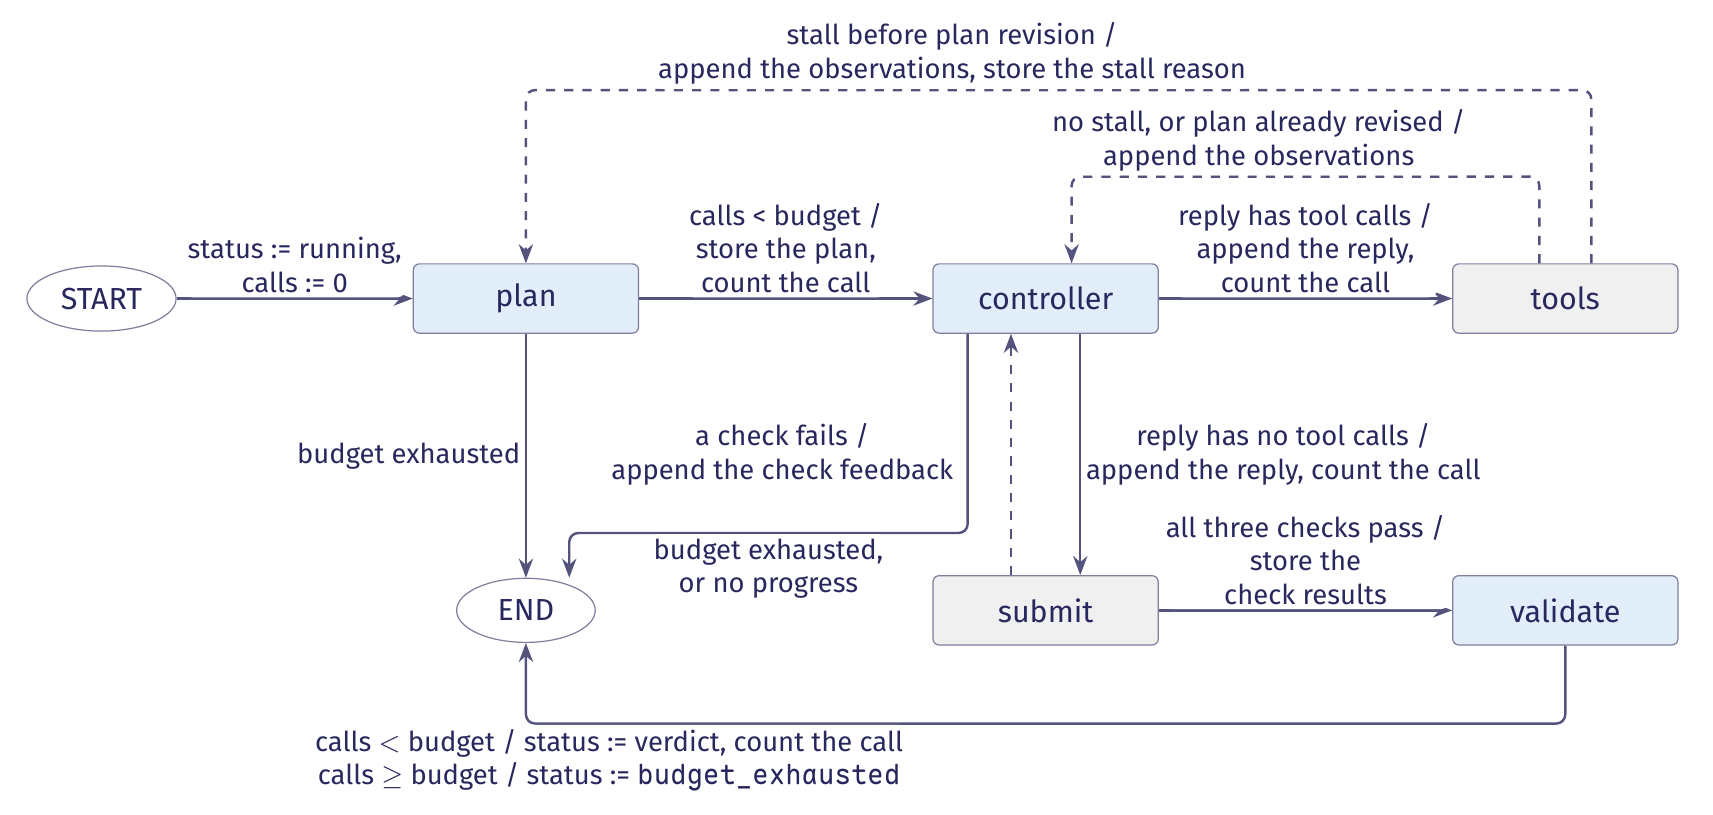
\includegraphics[width=0.92\textwidth]{figures/deck/675c3b4911.png}
  \caption{The planning agent as an extended state machine, with the nodes that call a model in blue
  and the nodes that run tools or checks in grey. Arrows carry guards and, after a slash, set
  actions, and the dashed arrows return to a location visited earlier.}
  \label{fig:machines-agent}
\end{figure*}

A run can visit the same location many times, and two visits to the controller can lead to
different next steps. What differs between the visits is the information the agent has kept, its
state.

\subsection{State, inputs and outputs}
\label{sec:machines-state}

The state of an agent is the information retained between steps that can affect what the agent does
next. Both the model and the runtime use that information. The controller's model reads its
instructions and the earlier observations, the results of tool calls as the runtime records them
(Lecture~2, Section~3), to choose an action. The runtime reads the call count, the number of model
calls made so far, to decide whether another model call is allowed.

\begin{definition}[State]
\label{def:machines-state}
State is the ``condition of the system at a particular point in time''. It ``[e]ncodes everything
about the past that influences the system's reaction to current input''
\citep[slide~10]{seshia2015discrete}.
\end{definition}

For an agent, the part of the past that reaches its next step through the state is what the agent
has kept: the messages exchanged with the model, the observations and the counters, among other
values. Anything else from the past can reach a later step only as an input.

An \textbf{input} is a result that the agent receives during a step: a model reply, a tool result
or the result of a check. The stored state alone does not determine an input. A model reply is an
input, so the same state can receive a different reply on another visit or in another run.

The files the agent works on lie outside the state in this description. The agent learns about them
through its tools and through the checks that \demoref{submit} runs. A tool's report about the files
enters the machine as an input, and the runtime then stores it as an observation. The result of an
edit, for example, records only that the edit was made, and a later read of that file reports the
new content.

An \textbf{output action} is the part of a transition that emits an output. The output is either a
request for an operation, such as running a tool, or the report of a terminal outcome, such as an
accepted patch.

The division between state and input separates what the program decides from what it receives. The
state determines which transitions are permitted. It does not determine which result arrives. Every
transition the agent can take is written in the program we designed, while the model, the tools and
the checks supply the inputs that select among them.

\subsection{Extended state machines and configurations}
\label{sec:machines-configurations}

An agent has a small number of control locations and a large amount of data, so we describe it as an
extended state machine. An \textbf{extended state machine} has finitely many control locations and a
set of variables that store data. Its transitions may read and write the variables.

\begin{definition}[Extended state machine]
\label{def:machines-extended}
``Extended state machines augment the FSM model with variables that may be read or written.''
\citep[slide~4]{seshia2015extended}
\end{definition}

In the quotation, FSM stands for finite-state machine, a state machine with finitely many states.

A \textbf{configuration} pairs the current control location with the current value of every
variable. It says where the run is and what the run holds. The variables hold the state of
\cref{sec:machines-state}. The configuration adds the control location, so one step can change the
location, the variables, or both.

For example, in the recorded run of \cref{sec:machines-trajectory}, just before the controller's
third model call, the configuration includes the following location and values:
\bi
\item \textbf{Location.} The run is at \demoref{controller}.
\item \textbf{\demoref{observations}.} Two tool results have been stored.
\item \textbf{\demoref{model\_calls}.} Three model calls have completed, one in \demoref{plan} and two
in \demoref{controller}.
\item \textbf{\demoref{status}.} The status is \demoref{running}. The status is the variable that
records whether the run is still going and, once it has ended, how it ended (Lecture~2).
\item \textbf{\demoref{messages}.} The variable holds the conversation so far.
\item \textbf{\demoref{plan}.} This variable, which shares its name with the location, holds the
plan: the list of steps the run intends to take. Lecture~2 called these steps plan steps, or
subgoals.
\ei
The configuration also holds the values of the other variables, such as the alert and the token
usage. In the same run, the controller is visited five times, and each visit has a different configuration
because the stored values have changed between visits.

Every run starts from the \textbf{initial configuration}. It pairs the first control location,
\demoref{plan}, with the starting values of the variables: the opening messages, counters at zero,
no observations and the status \demoref{running}. A \textbf{terminal configuration} is one from which
the runtime schedules no further step, so reaching it ends the run. The state then stores the reason
for ending, in the status.

An extended state machine can have finitely many control locations and infinitely many
configurations. How many configurations a location has depends on the values its variables can
take:
\bi
\item \textbf{A bounded counter.} The call budget, which Lecture~2 called the budget, is the most
model calls a run may make. If \demoref{model\_calls} were the only variable and the call budget were
$N$, the counter could hold the values $0$ through $N$. Each location would then have at most $N+1$
configurations, which is 41 for our budget of 40.
\item \textbf{An unbounded list.} If a list of messages can grow without a bound on its length, a
single control location can have infinitely many configurations.
\ei
A configuration is \textbf{reachable} when some run can arrive at it from the initial configuration.
When a machine has finitely many configurations, an analysis can examine every reachable one, for
example to show that no run arrives at an unsafe configuration. When a variable can take infinitely
many values, as the unbounded list can, a procedure that tries to list every reachable configuration
may never finish. The control locations and the guards (\cref{sec:machines-transitions}) still form
finite sets, and both are written in the program. An argument about the agent can therefore rest on
these finite sets and on properties of the variables, without listing configurations.
\Cref{sec:records} and \cref{sec:routing} argue in this way about the call budget.

\subsection{Transitions: guards, output actions and set actions}
\label{sec:machines-transitions}

In an extended state machine, a transition goes from one configuration to the next. Each transition
has a guard, an output action and a set action. The \textbf{guard} is a predicate, a true-or-false
test of the variables and the input, that states when the transition is allowed. The output action
emits the step's output (\cref{sec:machines-state}). The \textbf{set action} updates the variables.

Extended state machines label each arrow with the guard and the output action, separated by a slash,
and with the set action below them \citep[slide~5]{seshia2015extended}. We write one transition with
its input and the configurations before and after it:
\[
  (q, v) \xrightarrow{\;e\,;\; g \,/\, \mathit{out}\,;\, \mathit{set}\;} (q', v')
\]
At location $q$ with variable values $v$, input $e$ arrives. If the guard $g$ holds, the transition
emits $\mathit{out}$, applies $\mathit{set}$ to the variables, and moves to location $q'$ with values
$v'$.

\Cref{tab:machines-elements} gives each element of a transition its symbol and states what it is in
an agent. The guard is written $g(v, e)$ because it may test the stored variables, the new input, or
both.

\begin{table}[htbp]
  \caption{The elements of a transition in an agent's state machine, with the symbol used in the
  notation and what each element is in an agent.}
  \label{tab:machines-elements}
  \begin{adjustbox}{width=\linewidth}\begin{tabularx}{\linewidth}{L{0.24\linewidth}L{0.14\linewidth}X}
    \toprule
    \textbf{Element} & \textbf{Symbol} & \textbf{In an agent} \\
    \midrule
    \textbf{Control location} & $q$ & The computation ready to run: a model call, the execution of
      tools, or a check \\ \addlinespace
    \textbf{Variables} & $v$ & Messages, observations, a plan, counters, check results and a status,
      kept between steps \\ \addlinespace
    \textbf{Input} & $e$ & A result received during a step: a model reply, a tool result or a check
      result \\ \addlinespace
    \textbf{Guard} & $g(v, e)$ & A true-or-false test of the variables and the input, such as whether
      the reply requests a tool \\ \addlinespace
    \textbf{Output action} & $\mathit{out}$ & A request for an operation, or the report of a
      terminal outcome \\ \addlinespace
    \textbf{Set action} & $\mathit{set}$ & An update of the variables, such as storing a reply,
      extending the observations or incrementing a counter \\ \addlinespace
    \textbf{Initial configuration} & $(q_0, v_0)$ & The first control location with the starting
      values: opening messages, zero counters, no observations and the status \demoref{running} \\
      \addlinespace
    \textbf{Terminal configuration} & No symbol & A configuration from which no further computation is
      scheduled, with the reason for ending stored in the state \\
    \bottomrule
  \end{tabularx}\end{adjustbox}
\end{table}

The transition from the controller to the tools shows each element in code
(\cref{lst:machines-transition}). In the code, one transition is split between two functions. The
node \demoref{controller} receives the input and returns the set action. The routing function
\demoref{after\_controller} tests the guard. As in Lecture~2, Section~3, a routing function reads the
state after a node has finished and returns the name of the next location.

\noindent\begin{minipage}{\linewidth}
\begin{lstlisting}[basicstyle=\ttfamily\footnotesize, caption={Illustrative code for the transition from the controller to the tools: the node receives the input and returns the set action, and the routing function tests the guard.}, label=lst:machines-transition]
def controller(state):
    # (the budget and stall checks that run first are omitted)
    reply = call_model(state["messages"])  # the input e
    return {"messages": [reply],           # set: append the reply
            "model_calls": 1,              # set: add one call
            "usage": usage_of(reply)}      # set: add the usage

def after_controller(state):
    if state["status"] != RUNNING:
        return END
    if state["messages"][-1].tool_calls:   # the guard g
        return "tools"
    return "submit"
\end{lstlisting}
\end{minipage}

The elements of this transition are the following:
\bi
\item \textbf{Input.} The model's reply is the input $e$. It arrives from the model during the step.
\item \textbf{Set action.} The node returns the reply, the number 1 and the reply's token usage. The
runtime appends the reply to the stored messages, adds 1 to the stored \demoref{model\_calls}, and
adds the usage to a running total. How the runtime merges a returned value with a stored one is the
subject of \cref{sec:records}.
\item \textbf{Guard.} The test \demoref{state["messages"][-1].tool\_calls} is the guard. In the code
it runs after the set action, and it reads the reply from its stored copy, the last message. The
order makes no difference here, because both transitions that leave the controller after a model
call apply the same set action.
\item \textbf{Output action.} The transition requests that the tools be executed.
\ei
The first test in \demoref{after\_controller} handles a run that the runtime has already stopped.
If the status is no longer \demoref{running}, the function returns \demoref{END}
(\cref{sec:machines-planning}).

\subsection{Behaviors, computation trees and traces}
\label{sec:machines-behaviors}

A \textbf{behavior} is the sequence of steps that a run takes, leaving out stuttering steps. A
\textbf{stuttering step} is a step with no input, no change of state and no output. Such a step
changes nothing that can be observed, so leaving it out loses no information. Two descriptions of a
run that differ only in stuttering steps describe the same behavior.

A \textbf{computation tree} represents every possible behavior from the initial configuration. Its
root is the initial configuration. Each tree node is the configuration on one visit to a control
location, and the children of a tree node are the configurations that one step can reach from it. A
run follows one path from the root.

A machine is \textbf{deterministic} when, in every configuration, each input enables exactly one
transition. A machine is \textbf{nondeterministic} when it can allow several next steps for the same
input. For a fixed sequence of inputs, a deterministic machine therefore exhibits a single behavior.
A nondeterministic machine exhibits a set of behaviors, so its computation tree branches even when
the inputs are fixed \citep[slides~29 and~36]{seshia2015discrete}.

The planning agent is deterministic in this sense. Given a configuration and an input, its guards
select one transition. Its computation tree still branches, because the inputs can differ: the model
can return a different reply, and a check can pass or fail. Every branch in the planning agent's tree
is a point where an input can differ.

A deterministic machine is a different notion from the deterministic environment of Lecture~2. The
environment is deterministic because the same tool call on unchanged files returns the same result.
Determinism of the machine is a property of its transition rule. The model's replies are inputs to
the machine, and neither notion makes them repeatable.

\begin{definition}[Trace]
\label{def:machines-trace}
``A trace is the record of inputs, states, and outputs in a behavior.''
\citep[slide~8]{seshia2015extended}
\end{definition}

The state and the trace hold different information. The state holds the run's current information
only. The trace records the run's inputs, states and outputs over time.

The runtime's trace, which Lecture~2 introduced as the log of events the runtime writes during a run,
is a trace in the sense of \cref{def:machines-trace}. It is restricted to the inputs, state values and
outputs that the runtime chooses to log. An \textbf{event} is one entry that the runtime appends to
the trace. Every event has one of the following kinds:
\bi
\item \textbf{\demoref{model\_call}.} The event records one model call, the node that made it, and the
tool calls that the reply requested.
\item \textbf{\demoref{routing}.} The event records a routing decision, its destination, and the
\demoref{by} field of Lecture~2, which names whether the model or the runtime supplied the value that
the routing function tested.
\item \textbf{\demoref{tool\_request}.} The event records a tool call that the model requested.
\item \textbf{\demoref{tool\_result}.} The event records the outcome of a tool call.
\item \textbf{\demoref{state\_change}.} The event records a change that a node made to the state,
such as the results of the checks, or, after an exception escapes the run, the name of that
exception (\cref{sec:routing}).
\item \textbf{\demoref{terminal}.} The event states how the run ended, and it is normally the
trace's last event (\cref{sec:routing}).
\ei

The events written when the planning agent submits a patch show what the trace contains. In the
recorded run of \cref{sec:machines-trajectory}, the controller's last reply requested no tools, and
the trace then holds the following events, in order:
\be
\item A \demoref{model\_call} event records the controller's call, with an empty list of tool calls.
\item A \demoref{routing} event records the decision to go to \demoref{submit}, with \demoref{by}
set to \demoref{model}, because the reply's lack of tool calls selected it.
\item A \demoref{state\_change} event records the results of the three checks in \demoref{submit},
all of which passed.
\item A \demoref{routing} event records the decision to go to \demoref{validate}, with \demoref{by}
set to \demoref{runtime}, because the check results selected it.
\ee
These events contain a recorded input (the reply's empty list of tool calls), recorded state values
(the check results) and recorded decisions.

The trace matters because the state does not outlive the program. The state lives in the memory of
the running program, and when the program exits, any state that was not saved is lost. The trace and
the files the agent changed can remain. After a run, they are what is left as evidence of what
happened in it. \Cref{sec:records} discusses what saving the state itself would require.

\subsection{The planning agent as an extended state machine}
\label{sec:machines-planning}

\Cref{fig:machines-agent} draws the planning agent as an extended state machine, with each arrow
labeled by its guard and set action. Output actions are omitted. In the labels, \emph{calls} stands
for the call count, the variable \demoref{model\_calls}, and \emph{budget} for the call budget of 40.
The arrow from \demoref{START} carries only a set action, and the other arrows without a slash carry
only a guard. The label ``a check fails / append the check feedback'' belongs to the dashed arrow
from \demoref{submit} up to \demoref{controller}. We read the machine in parts: the forward path that
an accepted run follows, the feedback edges that return to an earlier location, and the exits that
end a run.

\paragraph{The forward path.}
An accepted run moves from \demoref{START} through \demoref{plan}, \demoref{controller},
\demoref{submit} and \demoref{validate} to \demoref{END}, with visits to \demoref{tools} along the
way. The transitions on this path are the following:
\be
\item \textbf{Start.} The arrow from \demoref{START} carries the initial set action: the status
becomes \demoref{running} and the call count becomes zero.
\item \textbf{Plan.} If the call count is below the budget, the planner calls the model, stores the
plan and counts the call.
\item \textbf{Controller.} If the call count is below the budget, the controller calls the model,
appends the reply and counts the call. If the reply has tool calls, the run goes to
\demoref{tools}. If it has none, the run goes to \demoref{submit}.
\item \textbf{Submit.} If all three checks pass, \demoref{submit} stores the check results and the
run goes to \demoref{validate}.
\item \textbf{Validate.} If the call count is below the budget, the validator calls the model, stores
its verdict in the status and counts the call. The run then ends.
\ee

The plan is stored in the state, and it reaches the controller as a message (Lecture~2, Section~4).
The controller's model reads it. No routing function reads it. While the status is
\demoref{running}, the routing after the controller depends only on whether the reply requests
tools. The plan's subgoals are therefore carried out through the control locations already in the
graph. No location corresponds to a subgoal, and no guard tests one.

The checks in \demoref{submit} are a gate in front of the validator. Only a patch that passes all
three reaches \demoref{validate}, and only the validator can end a run with an accepted patch.

\paragraph{The feedback edges.}
A \textbf{feedback edge} sends execution back to a location that the run has visited earlier.
Lecture~2 called such an edge a back edge. \Cref{fig:machines-agent} draws the planning agent's
feedback edges dashed:
\bi
\item \textbf{Tool loop.} The tool loop returns execution from \demoref{tools} to
\demoref{controller} when there is no stall, or when the plan has already been revised. Its set
action appends the tool results to the observations. This edge gives every observation back to the
model, as in the reactive loop of Lecture~2. After a revision, a run that stalls again also takes
this edge, and the controller's check then ends the run.
\item \textbf{Revision.} A revision returns execution from \demoref{tools} to \demoref{plan} after
the first stall. Its set action appends the observations and stores the reason for the stall, and the
planner then writes a new plan.
\item \textbf{Repair.} A repair returns execution from \demoref{submit} to \demoref{controller} when a
check fails. Its set action adds the reasons for the failure to the messages, so the controller's
model can write another patch.
\ei
Besides the tool loop, two feedback edges respond to failures: revision and repair. \Cref{sec:routing}
gives each feedback edge its trigger, the information it passes back, and the bound on how often it
can be taken.

The stall check that triggers a revision refines the stall check of Lecture~2. It reads the last three
observations since the latest revision of the plan, or since the start of the run if there has been
none. It reports a stall when all three are identical and none of them records a successful edit. A
successful edit changes the files, so three observations that include one do not count as a stall.

Until the plan has been revised, the \demoref{tools} node runs this check after recording each new
observation. On the first stall, it stores the reason in the variable \demoref{failed\_step}, and the
routing after \demoref{tools} sends the run to \demoref{plan}. After revising the plan, the planner
stores the number of observations at that moment in \demoref{replanned\_at}. Later stall checks
start from that position, so the stall that caused the revision cannot count against the revised
plan (\cref{sec:records}). After the revision, the \demoref{tools} node no longer runs the check.
The controller runs it before each of its model calls, so the controller detects a second stall.

\paragraph{The exits.}
A run reaches \demoref{END} through one of the following exits, and each sets the status on the way:
\bi
\item \textbf{The budget.} Before each model call, \demoref{plan}, \demoref{controller} and
\demoref{validate} compare the call count with the budget. If the count has reached 40, the node
makes no call and the run ends with \demoref{budget\_exhausted}. Lecture~2 described this check only
for the controller. Every node that calls a model performs it.
\item \textbf{A second stall.} If the run stalls again after a revision, the controller's check
before its next call ends the run with \demoref{no\_progress}.
\item \textbf{The verdict.} The validator's verdict, \demoref{accepted} or \demoref{rejected},
becomes the status, and the run ends in both cases.
\ei
Each exit leads to a terminal configuration: the location \demoref{END}, with a status that records
why the run ended. \Cref{sec:routing} examines what each ending establishes about the run.

\subsection{A run as a trajectory}
\label{sec:machines-trajectory}

A trajectory is the path a run follows through the computation tree. Lecture~2 used the word for
the record of the steps a run took. The computation tree makes the idea precise: a trajectory is one
path from the root, and each tree node on it is the configuration on one visit to a control
location. The behavior of a run is its sequence of steps, its trajectory is that sequence drawn as a
path in the computation tree, and its trace is the record of the inputs, states and outputs along
it.

We follow a recorded run of the planning agent on the worked alert of Lecture~2, a possible SQL
injection in one test case of OWASP BenchmarkPython. The run took the forward path with four rounds
through the tools. A round is one pass from the controller through \demoref{tools} and back, which
is one turn of the loop in the terms of Lecture~2:
\be
\item The planner wrote the plan.
\item The controller requested a tool four times, and \demoref{tools} ran it each time:
\demoref{read\_file}, \demoref{search}, \demoref{read\_file} and \demoref{edit}.
\item On its fifth visit, the controller replied without tool calls, and the run went to
\demoref{submit}.
\item All three checks passed, and the run went to \demoref{validate}.
\item The validator accepted the patch, and the run ended with the status \demoref{accepted}.
\ee
The run made seven model calls: one in \demoref{plan}, five in \demoref{controller} and one in
\demoref{validate}.

\begin{figure}[t]
  \centering
  \begin{adjustbox}{max width=\linewidth}
  \begin{tikzpicture}[
    every node/.style={font=\sffamily\footnotesize},
    rec/.style={draw=ibmblue, fill=ibmblue!8, line width=.8pt, rounded corners=2pt,
                minimum width=22mm, minimum height=7.5mm, align=center, inner sep=2pt},
    alt/.style={draw=black!40, text=black!65, fill=black!3, rounded corners=2pt,
                minimum width=22mm, minimum height=7.5mm, align=center, inner sep=2pt},
    dots/.style={text=black!55},
    hit/.style={-{Stealth[length=1.8mm]}, line width=1.1pt, draw=ibmblue},
    may/.style={-{Stealth[length=1.8mm]}, densely dotted, line width=.7pt, draw=black!50},
    el/.style={font=\sffamily\scriptsize, fill=white, inner sep=1pt, align=center, text=black!75}
  ]
    % recorded path, centre column
    \node[rec] (plan) at (0,0)      {\textbf{plan}\\0 calls};
    \node[rec] (c1)   at (0,-1.2)   {\textbf{controller}\\1 call};
    \node[rec] (t1)   at (0,-2.4)   {\textbf{tools}: \texttt{read\_file}\\2 calls};
    \node[rec] (c2)   at (0,-3.6)   {\textbf{controller}\\2 calls};
    \node[rec] (t2)   at (0,-4.8)   {\textbf{tools}: \texttt{search}\\3 calls};
    \node[rec] (mid)  at (0,-6.0)
      {two more rounds of controller\\and tools: \texttt{read\_file}, \texttt{edit}};
    \node[rec] (c5)   at (0,-7.2)   {\textbf{controller}\\5 calls};
    \node[rec] (s6)   at (0,-8.4)   {\textbf{submit}\\6 calls};
    \node[rec] (v6)   at (0,-9.9)   {\textbf{validate}\\6 calls};
    \node[rec] (acc)  at (0,-11.0)  {\textbf{END}: \texttt{accepted}\\7 calls};

    % alternatives
    \node[alt] (s2)   at (3.25,-2.4)  {\textbf{submit}\\2 calls};
    \node[dots] (s2d) at (3.25,-3.45)  {$\cdots$};
    \node[alt] (s3)   at (3.25,-4.8)  {\textbf{submit}\\3 calls};
    \node[dots] (s3d) at (3.25,-5.85)  {$\cdots$};
    \node[alt] (t6)   at (-3.25,-8.4) {\textbf{tools}\\6 calls};
    \node[alt] (exh)  at (-3.25,-9.9)
      {\textbf{END}:\\\texttt{budget\_exhausted}\\40 calls};
    \node[alt] (r6)   at (3.25,-8.4)  {\textbf{controller}\\6 calls};
    \node[dots] (r6d) at (3.25,-9.45)  {$\cdots$};
    \node[alt] (rej)  at (-3.25,-11.0) {\textbf{END}: \texttt{rejected}\\7 calls};

    % recorded edges
    \draw[hit] (plan) -- (c1);
    \draw[hit] (c1) -- node[el, left=1pt] {tool calls} (t1);
    \draw[hit] (t1) -- node[el, left=1pt] {no stall} (c2);
    \draw[hit] (c2) -- node[el, left=1pt] {tool calls} (t2);
    \draw[hit] (t2) -- node[el, left=1pt] {no stall} (mid);
    \draw[hit] (mid) -- (c5);
    \draw[hit] (c5) -- node[el, right=1pt] {no tool calls} (s6);
    \draw[hit] (s6) -- node[el, right=1pt] {checks pass} (v6);
    \draw[hit] (v6) -- node[el, right=1pt] {accepted} (acc);

    % alternative edges
    \draw[may] (c1) -- node[el, sloped, above] {no tool calls} (s2);
    \draw[may] (s2) -- (s2d);
    \draw[may] (c2) -- node[el, sloped, above] {no tool calls} (s3);
    \draw[may] (s3) -- (s3d);
    \draw[may] (c5) -- node[el, sloped, above] {tool calls} (t6);
    \draw[may] (t6) -- node[el, right=1pt, align=left] {more rounds,\\until 40 calls} (exh);
    \draw[may] (s6) -- node[el, above=1pt] {a check\\fails} (r6);
    \draw[may] (r6) -- (r6d);
    \draw[may] (v6) -- node[el, sloped, above] {rejected} (rej);

    \node[el, text=black!60, anchor=west] at (1.25,0) {initial configuration};
  \end{tikzpicture}
  \end{adjustbox}
  \caption{Part of the planning agent's computation tree. The blue path is the trajectory of the
  recorded run, and the grey nodes are configurations that other inputs would have reached. Each
  tree node shows its control location and the number of model calls completed on reaching it.}
  \label{fig:machines-tree}
\end{figure}

\Cref{fig:machines-tree} places this run in the computation tree. Each tree node shows a control
location and the number of model calls completed on reaching it. The blue path is the recorded
trajectory, and its middle box stands for two more rounds through the controller and \demoref{tools},
drawn as one box. The tree branches at each visit to the controller (tool calls or none), at
\demoref{submit} (all checks pass or a check fails) and at \demoref{validate} (accepted or
rejected). A visit to \demoref{tools} can also branch, because a stall sends the run to
\demoref{plan}. The figure does not draw that branch. The grey branch that leaves the controller's
fifth visit shows a run that keeps requesting tools until the call count reaches the budget. Each
$\cdots$ marks a part of the tree that the figure leaves out.

The machine of \cref{fig:machines-agent} and the tree of \cref{fig:machines-tree} answer different
questions:
\bi
\item \textbf{The machine.} It shows which transitions are permitted. It has one node per control
location, so the controller appears once.
\item \textbf{The tree.} It shows which sequences of transitions are possible from the initial
configuration. It has one tree node per visit, so the controller appears five times on the recorded
path, each time with a different configuration.
\ei

Another run on the same alert can follow a different path through the same tree. The graph and its
guards are the same in every run. The model's replies are inputs, and a different reply selects a
different child.

\subsection{What the trace records and what we infer}
\label{sec:machines-recorded}

The runtime's trace records selected inputs, outputs and state values, so some facts about a run are
recorded and others must be inferred. The trace omits the following information:
\bi
\item \textbf{Tool output.} A successful \demoref{tool\_result} event records the length of the
result in characters. It omits the text that the tool returned.
\item \textbf{Some routing decisions.} The trace has no routing event for the moves from
\demoref{tools} to \demoref{controller} and from \demoref{plan} to \demoref{controller}. We infer
these moves from the controller's next \demoref{model\_call} event and the transition rules.
\item \textbf{The call count.} The trace does not record \demoref{model\_calls}. We reconstruct it by
starting at zero and adding one for each \demoref{model\_call} event.
\ei

Every claim about a run must therefore say whether the trace records it directly or whether it is
inferred from recorded events and the transition rules. Some facts are neither recorded nor
inferable. In the recorded run of \cref{sec:machines-trajectory}, the distinction applies as follows:
\bi
\item \textbf{Recorded.} The results of the three checks are recorded in a \demoref{state\_change}
event, and the decision to go to \demoref{validate} in a \demoref{routing} event.
\item \textbf{Inferred.} The call count of seven is inferred by counting \demoref{model\_call}
events. Each return from \demoref{tools} to \demoref{controller} is inferred from the controller's
next call.
\item \textbf{Absent.} The text that each \demoref{read\_file} returned is not in the trace. A claim
about what the model read cannot rest on the trace alone.
\ei

An inference depends on the transition rules it uses and on the events it starts from. If a rule is
wrong or an event is missing, the inference can be wrong. \Cref{sec:routing} examines endings in which
the event that would settle how a run ended is missing.

\subsection*{Key points}
\bi
\item A state machine is a simplified description of an agent that omits the prompts, the model and
the tool code, and specifies states, inputs, outputs, an initial configuration, a transition rule
and, for a workflow meant to end, terminal configurations.
\item The state is the information retained between steps that can affect the next step, and model
replies, tool results and check results are inputs that arrive during a step and select among the
transitions the state permits.
\item An extended state machine pairs finitely many control locations with variables, and a
configuration is a location together with the value of every variable, so an unbounded message list
can give one location infinitely many configurations.
\item A transition $(q, v) \xrightarrow{e;\, g/\mathit{out};\, \mathit{set}} (q', v')$ is allowed
when its guard $g$ holds for the variables and the input $e$, and it then emits $\mathit{out}$,
applies $\mathit{set}$ and moves to $q'$.
\item The planning agent is deterministic because its guards select one transition for each
configuration and input, so its computation tree branches only where an input can differ, and a
run's trajectory is one path through that tree.
\item In the planning agent, the plan reaches the controller only as a message that no guard reads,
the feedback edges are the tool loop, revision and repair, and a run ends when the call count
reaches the budget of 40, at a second stall, or with the validator's verdict.
\item Unsaved state is lost when the program exits, and the trace that remains records only selected
inputs, outputs and state values, so every claim about a run must say whether it is recorded or
inferred from recorded events and the transition rules.
\ei

\section{State, records and reducers}
\label{sec:records}

\Cref{sec:machines} described the planning agent as an extended state machine, in which a
configuration pairs a control location with the current value of every variable. This section shows
how the runtime stores those values, how one step changes them, and how long each stored value stays
valid. It also separates the stored values from what a model call receives and from what survives
the process, proves that the call budget holds at every step, and shows how the graph is built. The
routing and stopping rules of \cref{sec:routing} read these stored values, so they rest on the
mechanisms described here.

\subsection{State records and schemas}
\label{sec:records-schema}

A \textbf{state record} stores the information that an agent retains between steps as named fields
with their current values. A \textbf{field} is one named entry of the record. \Cref{sec:machines}
called the retained information the state and called its parts variables, so the record is the
stored form of the state and each field holds the value of one variable. For example, the field
\demoref{model\_calls} with the value 2 records that two model calls have completed.

The runtime keeps the control location and the variable values of a configuration in different
places. The runtime itself
tracks the control location, which identifies the computation to run next. The state record holds
the values of the variables, such as the messages exchanged with the model and
\demoref{model\_calls}. The graph of the agent describes control flow, that is, which computation
may run next. The record supplies the values that those computations read.

Each run has its own record, which holds the current values for that run. Every node of the run
reads the same record, so the record is the state that the nodes share.

The fields of the record are declared in a state schema, which, as in Lecture~2, lists the fields
the state contains and their types. Our agents are built with LangGraph, a library for writing
programs as graphs of nodes and edges. LangGraph documents a \demoref{TypedDict} class as the main
way to write a schema \citep{langgraph-graph-api}. A \demoref{TypedDict} is a Python dictionary type
with a fixed set of keys and a declared type for the value of each key \citep{pep589}. Each key of
our schema names one field.

Our schema is the class \demoref{AgentState}. LangGraph builds a graph with its class
\demoref{StateGraph}, and the call \demoref{StateGraph(AgentState)} creates a graph whose shared
state has the fields that \demoref{AgentState} declares.

The schema and the record play different roles. The schema declares the names and types of the
fields, and it is the same for every run. The record holds values, and they change from step to
step. A node never returns a whole record. It returns only the fields that it changes
(\cref{sec:records-updates}). Once those fields are merged into the record, routing functions read
the updated record to select the next node (\cref{sec:routing}).

\subsection{Partial updates}
\label{sec:records-updates}

A node changes the record by returning a partial update, which the runtime merges into the record
one field at a time. A \textbf{partial update} is a mapping from the fields that a node changes to
the values it returns for them.

A \textbf{reducer} is the rule that merges the value stored in a field with the value that a node
returns for that field. Every field has a reducer. A field whose declaration names none takes the
default reducer, which replaces the stored value with the returned one \citep{langgraph-graph-api}.
\Cref{sec:records-reducers} describes the kinds of reducer our agents use.

One step proceeds as follows:
\be
\item The runtime passes the current record, written $s_t$, to the node.
\item While it runs, the node receives an input, written $e_t$: a model reply, a tool result or a
check result.
\item The node returns a partial update, written $u_t$.
\item For each field in $u_t$, the runtime calls that field's reducer. The stored value is the
reducer's left argument, and the returned value is its right argument.
\item The merged record is the next state, $s_{t+1}$.
\ee

\Cref{fig:records-update} draws these steps. The dashed arc carries the stored value from $s_t$
straight to the reducer, so the left argument never passes through the node.

\begin{figure}[htbp]
  \centering
  \begin{adjustbox}{width=\linewidth}
  \begin{tikzpicture}[node distance=6mm and 3mm]
    \node[rnode] (s0) {state $s_t$};
    \node[mnode, right=of s0] (node) {node};
    \node[gnode, right=of node] (upd) {partial\\update $u_t$};
    \node[rnode, right=11mm of upd] (red) {reducer,\\one per field};
    \node[rnode, right=of red] (s1) {state $s_{t+1}$};
    \node[tnode, align=center, below=7mm of node] (ext) {model reply, tool result\\or check result $e_t$};
    \draw[flow] (s0) -- (node);
    \draw[flow] (node) -- (upd);
    \draw[flow] (upd) -- node[lab, below] {right\\argument} (red);
    \draw[flow] (red) -- (s1);
    \draw[flow] (ext) -- (node);
    \draw[back] (s0.north) to[out=35, in=145] node[lab, above] {left argument} (red.north);
  \end{tikzpicture}
  \end{adjustbox}
  \caption{One step of a run. The node reads the stored state and an input, and returns a partial
  update. For each field in the update, the field's reducer merges the stored value (left argument)
  with the returned value (right argument), and the result is the next state.}
  \label{fig:records-update}
\end{figure}

For a field $f$ with reducer $r_f$, where $s_t[f]$ is the value of $f$ in the record $s_t$, the
merge follows one rule:
\begin{equation*}
  s_{t+1}[f] =
  \begin{cases}
    r_f\bigl(s_t[f],\, u_t[f]\bigr) & \text{if } u_t \text{ contains } f,\\[2pt]
    s_t[f] & \text{otherwise.}
  \end{cases}
\end{equation*}
A field omitted from the partial update keeps its stored value. A node therefore never has to copy
the fields it leaves unchanged. It also cannot erase a field by leaving it out.

A node controls only the value it returns. The field's reducer, which the schema declares, fixes how
that value combines with the stored one. The one exception is an explicit overwrite, which bypasses
the reducer (\cref{sec:records-reducers}).

In the terms of \cref{sec:machines}, the partial update and the reducers together carry out the set
action of the transition, the update of the variables. The run then moves to its next control
location, which a routing function selects by reading the merged record (\cref{sec:routing}).

\subsection{The controller's return sites}
\label{sec:records-controller}

The controller ends every visit with a partial update that either stops the run with a status or
records one model call: the reply, the completed call and the reply's token usage. We call each
\demoref{return} statement of a node a \textbf{return site}, and each return site gives the runtime
one partial update. The controller's return sites, in the order its code reaches them, are the
following:
\bi
\item \textbf{Budget.} If the call budget is spent, the controller returns only the field
\demoref{status}, set to \demoref{budget\_exhausted}.
\item \textbf{Stall.} If the stall check finds that the run has stalled, the controller returns only
\demoref{status}, set to \demoref{no\_progress}.
\item \textbf{Model call.} Otherwise, the controller calls the model once. It returns the reply in
\demoref{messages}, one completed call in \demoref{model\_calls}, and the reply's token counts in
\demoref{usage}.
\ei

The first test is the \textbf{admission check}, the comparison of \demoref{model\_calls} with the
budget before each model call (\cref{sec:records-context}). Both stopping tests run before the model
call, so a run that must stop makes no further call. A routing function then reads the status and
ends the run (\cref{sec:routing}).

\Cref{fig:records-controller} applies these return sites to the reactive loop of Lecture~2,
Section~3. Its record is smaller, with ten fields, and its controller has the same return sites in
the same order as the planning agent's. After a model call, the update changes \demoref{messages},
\demoref{model\_calls} and \demoref{usage}. The reducer of \demoref{messages} appends the reply, the
reducer of \demoref{model\_calls} adds one, and the reducer of \demoref{usage} adds each token count
to its running total. A stopping return site changes only \demoref{status}. That field declares no
reducer, so it takes the default, and the returned string replaces the stored one.

\begin{figure*}[t]
  \centering
  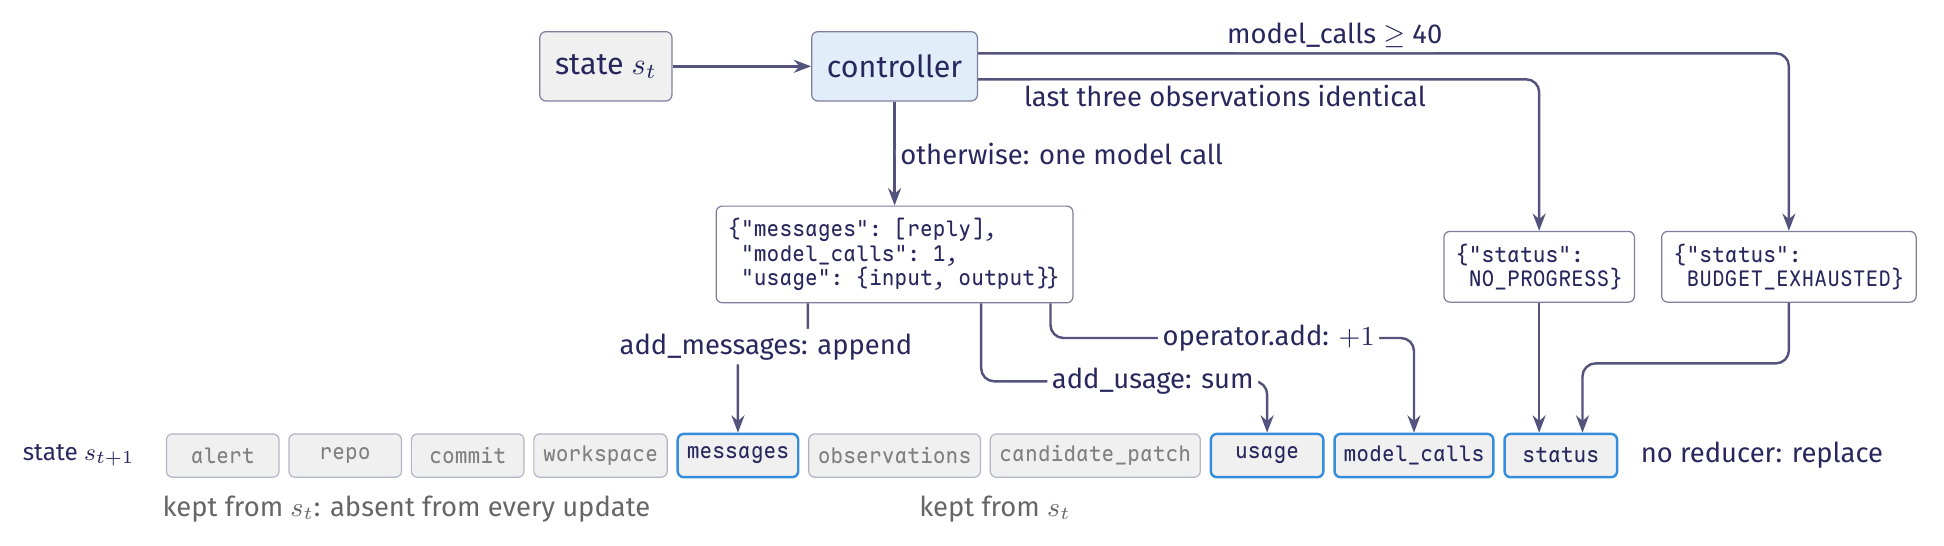
\includegraphics[width=\textwidth]{figures/deck/ee17da9c44.png}
  \caption{The return sites of the reactive loop's controller, applied to its ten-field record. Each
  of the two stopping paths returns only a status. The path through a model call returns the reply,
  one completed call and the reply's token usage (shown with its input and output counts), and each
  of those fields is merged by its reducer. Fields in grey appear in no update and keep their
  stored values.}
  \label{fig:records-controller}
\end{figure*}

The remaining fields, \demoref{alert}, \demoref{repo}, \demoref{commit}, \demoref{workspace},
\demoref{observations} and \demoref{candidate\_patch}, are absent from every update the controller
returns. They keep their stored values after every visit to the controller.

\Cref{lst:records-controller} shows the planning agent's controller. The listing is illustrative and
leaves out the event that the controller writes to the trace.

This controller differs from the reactive loop's in its stall check, which reads only the
observations recorded since the latest revision of the plan, or since the start of the run if the
plan has not been revised. The function \demoref{planning\_window} selects them
(\cref{sec:records-lifetimes}). The tools node detects the first stall and sends the run to the plan
node. In the planning agent, this return site therefore ends the run only when the run stalls again
after a revision.

\noindent\begin{minipage}{\linewidth}
\begin{lstlisting}[basicstyle=\ttfamily\footnotesize, caption={Illustrative code for the planning
agent's controller node. Each \texttt{return} is one return site.}, label=lst:records-controller]
def controller(state):
    stop = admission_check(state)        # budget
    if stop:
        return stop
    if stalled(planning_window(state), limit=3):
        return {"status": NO_PROGRESS}   # stall
    reply = call_model(state["messages"])
    return {"messages": [reply],         # model call
            "model_calls": 1,
            "usage": usage_of(reply)}
\end{lstlisting}
\end{minipage}

The first return site passes on whatever the admission check returns (\cref{lst:records-admission}).
When the budget is spent, the check returns a status update that ends the run. Otherwise it returns
\demoref{None}, and the controller goes on to the stall check.

The second return site applies \demoref{stalled} to the observations that
\demoref{planning\_window} selects. With \demoref{limit=3}, it reports a stall when the last three of
them are identical and none records a successful edit. The last return site reports one completed
call as \demoref{"model\_calls": 1}. The reducer adds this one to the stored count, so a stored count
of 2 becomes 3.

\subsection{Model context, runtime state and durable state}
\label{sec:records-context}

Information about a run exists as model context, runtime state and durable state, which differ in
what they hold, who reads them and how long they last. The \textbf{model context} is what one model
call receives: the instructions, a selection of the history, and observations. Lecture~2 called it
the model's context.

The \textbf{runtime state} is the set of fields that the running process retains between steps,
including counters that the model never sees. It is the state record of \cref{sec:records-schema},
held in the memory of the running process. We say runtime state when we contrast the record with the
model context and the durable state.

The \textbf{durable state} is state that outlives the process, in a form that another process can
load to resume the run. \Cref{tab:records-context} compares the three. Its last column shows the
difference that matters for resuming: only the durable state can be loaded by a new runtime process.

\begin{table}[htbp]
  \caption{Model context, runtime state and durable state: what each holds, and who reads it.}
  \label{tab:records-context}
  \begin{adjustbox}{width=\linewidth}\begin{tabularx}{\linewidth}{L{0.22\linewidth}XL{0.27\linewidth}}
    \toprule
    \textbf{State or context} & \textbf{What it holds} & \textbf{Who reads it} \\
    \midrule
    \textbf{Model context} & The instructions, selected history and observations supplied to one
    model call & The model \\
    \textbf{Runtime state} & The fields retained between steps, including counters that the model
    never sees & Nodes, routing functions and limit checks \\
    \textbf{Durable state} & State that survives the process, in a form another process can load to
    resume the run & A new runtime process \\
    \bottomrule
  \end{tabularx}\end{adjustbox}
\end{table}

For each model call, the runtime builds the model context from the runtime state. The controller
passes the conversation stored in \demoref{messages} to the model (\cref{lst:records-controller}).
The validator's context is built from other fields: the alert, the patch, the check results and
the observations (Lecture~2, Section~4). It never includes the conversation. A model context is
therefore a selection from the runtime state, made separately for each call.

To resume a run after its process exits, the runtime must have saved enough state to reconstruct
the execution. A \textbf{checkpointer} is the component that saves the runtime state as checkpoints
\citep{langgraph-persistence}. Lecture~2 called such saved progress a checkpoint. A checkpointer
that writes its checkpoints to a file or a database produces durable state, which a new process can
load to continue the run. One that keeps them in memory loses them when the process exits. Our
graphs are compiled without a checkpointer and keep their state in memory. When the process exits, the record is lost (\cref{sec:machines}).

The trace survives the process, but a new process cannot rebuild the record from it. The trace
records selected events and omits values that resumption needs, such as the text that each tool
returned, which no event records (\cref{sec:machines}).

A saved record alone is also not enough to resume. The workspace files lie outside the state, so a
resumed run needs files that match the saved record. For example, if the record holds a patch that
was applied before the exit, the files must already contain that patch. A resumed run also needs the
pending work, that is, the steps that were scheduled but had not finished when the process exited.
A later unit of the course covers saved state, pending work and the workspace.

The call budget shows why the distinction between runtime state and model context matters. None of
the planning agent's prompts mentions the budget, so the budget is in no model context. The
admission check enforces it from the runtime state instead (\cref{lst:records-admission}). The
planning agent runs this check before every model call, in each node that calls the model:
\demoref{plan}, \demoref{controller} and \demoref{validate}.

\noindent\begin{minipage}{\linewidth}
\begin{lstlisting}[basicstyle=\ttfamily\footnotesize, caption={Illustrative code for the admission
check, which runs before every model call.}, label=lst:records-admission]
def admission_check(state) -> dict | None:
    if state["model_calls"] >= budget:   # budget = 40
        return {"status": BUDGET_EXHAUSTED}
    return None                          # call allowed
\end{lstlisting}
\end{minipage}

The check works even though the model never receives the budget. It is code in the runtime, and it
compares a counter that the model cannot write with a limit that we fix before the run starts.
Whatever the model writes, a call is issued only while \demoref{model\_calls} is below the budget.

\subsection{Reducers}
\label{sec:records-reducers}

A field's reducer decides how a returned value combines with the stored one, and our agents use
reducers that append, replace or accumulate. The kinds of reducer work as follows:
\bi
\item \textbf{Append.} The reducer adds the returned items to the end of the stored list, so later
nodes can read the full history. The fields \demoref{messages} and \demoref{observations} use append
reducers.
\item \textbf{Replace.} The reducer stores the returned value as the field's new value, as when the
plan node writes a revised plan. A field declared without a reducer takes replacement as its default
\citep{langgraph-graph-api}.
\item \textbf{Accumulate.} The reducer combines the returned contribution with the stored total, for
example by adding 1 to \demoref{model\_calls}. The field \demoref{usage} accumulates token counts in
the same way.
\ei

The schema attaches a reducer to a field with the form \demoref{Annotated[T, fn]}.
\demoref{Annotated} is the standard Python way to attach extra information to a type. Here
\demoref{T} names the field's type, and LangGraph reads \demoref{fn} as the field's reducer
(\cref{lst:records-schema}). A field written with its type alone, such as \demoref{status: str},
declares no reducer and takes the default, which replaces the stored value.

\noindent\begin{minipage}{\linewidth}
\begin{lstlisting}[basicstyle=\ttfamily\footnotesize, caption={Illustrative code for part of the
state schema, with the reducer of each field.}, label=lst:records-schema]
class AgentState(TypedDict, total=False):
    # other fields omitted
    messages: Annotated[list, add_messages]
    observations: Annotated[list, operator.add]
    usage: Annotated[Usage, add_usage]
    model_calls: Annotated[int, operator.add]
    status: str
\end{lstlisting}
\end{minipage}

Each field in the listing has the following reducer:
\bi
\item \textbf{\demoref{messages}.} The reducer \demoref{add\_messages} appends the returned messages
to the conversation. A returned message whose ID matches a stored message replaces that message
instead.
\item \textbf{\demoref{observations}.} The reducer \demoref{operator.add} joins two lists, so it
appends the returned observations.
\item \textbf{\demoref{usage}.} The reducer \demoref{add\_usage} accumulates. It keeps four separate
token counters and adds each returned count to the counter of the same kind. One counter holds cache
reads, the input tokens that the provider reuses from an earlier call, so they stay distinct from
fresh input tokens.
\item \textbf{\demoref{model\_calls}.} The same \demoref{operator.add} adds two integers here, so it
accumulates the count of completed calls.
\item \textbf{\demoref{status}.} The field declares no reducer, so it takes the default, and an
update replaces the stored string. If a node returns no status, the runtime keeps the previous one.
\ei
The words \demoref{total=False} in the class header declare that a dictionary of this type may
leave keys out \citep{pep589}. A partial update, which holds only some of the keys, therefore still
has the declared type.

Returning \demoref{[]} to an append reducer adds zero items, so the stored list keeps its contents.
Clearing a list such as \demoref{observations} therefore requires an explicit overwrite, which
bypasses the reducer and replaces the stored value.

LangGraph provides the wrapper \demoref{Overwrite} for this. A node that returns a value wrapped in
\demoref{Overwrite} replaces the stored list with that value. A reset of this kind should be
recorded as its own trace event. A reader of the trace otherwise assumes that the list only grows,
and cannot tell that earlier entries were discarded.

\subsection{Field lifetimes}
\label{sec:records-lifetimes}

A \textbf{field lifetime} is the interval during which later nodes may rely on a field's stored
value. The lifetime ends when a later step makes that value obsolete, for example when a revision of
the plan makes the old plan obsolete. A reducer decides only how a returned value is merged. It does
not decide how long later nodes may rely on that value.

\Cref{tab:records-lifetimes} defines the lifetimes. In our two agents, the identity fields are
\demoref{alert}, \demoref{repo}, \demoref{commit} and \demoref{workspace}. The run fields are
\demoref{messages}, \demoref{observations}, \demoref{usage} and \demoref{model\_calls}. The current
fields are \demoref{candidate\_patch}, \demoref{status}, \demoref{plan}, \demoref{checks} and
\demoref{validation}.

A \textbf{handoff field} holds a reason that one node leaves for another and is cleared after use,
here \demoref{failed\_step}. A \textbf{window field} holds an index where a window of a history
starts, here \demoref{replanned\_at}. An attempt is one try at producing an accepted patch. No field
of either agent has the attempt lifetime.

\Cref{fig:records-schemas} sets the two schemas side by side. The shading of each field gives its
lifetime from \cref{tab:records-lifetimes}, and a plus sign marks the fields that the planning agent
adds: \demoref{plan}, \demoref{failed\_step}, \demoref{replanned\_at}, \demoref{checks} and
\demoref{validation}.

The plan node writes \demoref{plan}, the submit node writes \demoref{checks}, and the validate node
writes \demoref{validation}. Each of these fields holds the latest value until its writer replaces
it. The tools node writes \demoref{failed\_step} for the plan node to read and clear. The index
\demoref{replanned\_at} marks where the observations made under the current plan begin.

\begin{figure*}[t]
  \centering
  \definecolor{recordslifeid}{HTML}{E4E4E4}
  \definecolor{recordsliferun}{HTML}{D0E2FF}
  \definecolor{recordslifecur}{HTML}{D4F0D4}
  \definecolor{recordslifehand}{HTML}{FFDFB8}
  \definecolor{recordslifewin}{HTML}{E6D6FF}
  \newcommand{\recordslf}[3][]{\par\noindent\hspace*{1em}\llap{\textbf{#1}\hspace{0.3em}}%
    {\setlength{\fboxsep}{0.6pt}\colorbox{#2}{\makebox[\dimexpr\linewidth-1em-1.2pt][l]%
    {\ttfamily\strut\hspace{1.5em}#3}}}\par}
  \newcommand{\recordslfhead}[1]{\par\noindent\hspace{1em}{\ttfamily\strut#1}\par}
  \newcommand{\recordslfgap}{\par\vspace{2pt}}
  \newcommand{\recordslfcap}[1]{\par\noindent{\sffamily\bfseries #1}\par\smallskip}
  \newcommand{\recordslfkey}[2]{{\setlength{\fboxsep}{1.5pt}\colorbox{#1}{#2}}}
  \setlength{\parskip}{0pt}%
  \footnotesize
  \begin{minipage}[t]{0.47\textwidth}
    \recordslfcap{The reactive loop}
    \recordslfhead{class AgentState(TypedDict, total=False):}
    \recordslf{recordslifeid}{alert: dict}
    \recordslf{recordslifeid}{repo: str}
    \recordslf{recordslifeid}{commit: str}
    \recordslf{recordslifeid}{workspace: str}
    \recordslfgap
    \recordslf{recordsliferun}{messages: Annotated[list, add\_messages]}
    \recordslf{recordsliferun}{observations: Annotated[list, operator.add]}
    \recordslf{recordslifecur}{candidate\_patch: str | None}
    \recordslf{recordsliferun}{usage: Annotated[Usage, add\_usage]}
    \recordslf{recordsliferun}{model\_calls: Annotated[int, operator.add]}
    \recordslf{recordslifecur}{status: str}
  \end{minipage}\hfill
  \begin{minipage}[t]{0.47\textwidth}
    \recordslfcap{The planning agent}
    \recordslfhead{class AgentState(TypedDict, total=False):}
    \recordslf{recordslifeid}{alert: dict}
    \recordslf{recordslifeid}{repo: str}
    \recordslf{recordslifeid}{commit: str}
    \recordslf{recordslifeid}{workspace: str}
    \recordslfgap
    \recordslf[+]{recordslifecur}{plan: list | None}
    \recordslf[+]{recordslifehand}{failed\_step: dict | None}
    \recordslf[+]{recordslifewin}{replanned\_at: int}
    \recordslf{recordsliferun}{messages: Annotated[list, add\_messages]}
    \recordslf{recordsliferun}{observations: Annotated[list, operator.add]}
    \recordslf{recordslifecur}{candidate\_patch: str | None}
    \recordslf[+]{recordslifecur}{checks: dict | None}
    \recordslf[+]{recordslifecur}{validation: dict | None}
    \recordslf{recordsliferun}{usage: Annotated[Usage, add\_usage]}
    \recordslf{recordsliferun}{model\_calls: Annotated[int, operator.add]}
    \recordslf{recordslifecur}{status: str}
  \end{minipage}

  \medskip
  {\sffamily Lifetime:\enspace
  \recordslfkey{recordslifeid}{identity}\enspace\recordslfkey{recordsliferun}{run}\enspace
  \recordslfkey{recordslifecur}{current}\enspace\recordslfkey{recordslifehand}{handoff}\enspace
  \recordslfkey{recordslifewin}{window}\qquad\textbf{+}\,new in the planning agent}
  \caption{The state schemas of the reactive loop and the planning agent. The shading of each field
  gives its lifetime, and a plus sign marks the fields that the planning agent adds.}
  \label{fig:records-schemas}
\end{figure*}

\begin{table}[htbp]
  \caption{The field lifetimes, with what each one means for the nodes that read and write the
  field.}
  \label{tab:records-lifetimes}
  \begin{adjustbox}{width=\linewidth}\begin{tabularx}{\linewidth}{L{0.2\linewidth}X}
    \toprule
    \textbf{Lifetime} & \textbf{Definition and use} \\
    \midrule
    \textbf{Identity} & Identity fields identify the task, the target and the workspace, and they
    remain unchanged. \\
    \textbf{Run} & Run fields retain histories and counters that grow throughout the run. \\
    \textbf{Current} & Current fields hold the latest plan, candidate, check result or status until
    the writer replaces them. \\
    \textbf{Handoff} & One node writes a reason for invoking another node. The receiving node reads
    that handoff field and clears it after acting. \\
    \textbf{Window} & An index field marks where a selected window of history begins. Checks read
    from that index onward while the complete history remains stored. \\
    \textbf{Attempt} & An attempt field holds the results of one attempt. Nodes clear it before a
    new attempt, so later steps cannot treat old results as current. \\
    \bottomrule
  \end{tabularx}\end{adjustbox}
\end{table}

The attempt lifetime is absent because neither agent starts a new attempt. In the planning agent,
a rejection by the validator ends the run, and the reactive loop has no validator. In both agents, a
patch that fails the checks returns to the controller for repair, but no field is cleared, and the
run continues as a single attempt. Neither schema
therefore needs fields that must be cleared before a new attempt.

\Cref{sec:routing} discusses a proposed new attempt after a rejection. If it were added, fields that
hold one attempt's results, such as the plan and the candidate patch, would become attempt fields.

The runtime merges updates according to reducers. It does not enforce lifetimes, so node code
must enforce them, by retaining, replacing or clearing each field when required. A reducer sees
only the stored value and the returned value. It cannot know that a revision has happened or that
a reason has been acted on.

Run fields must keep their values across attempts, which matters once a new attempt is added
(\cref{sec:routing}). The call count shows why. A counter that limits the whole run must keep its
total. If \demoref{model\_calls} were reset to zero at a new attempt, later calls would ignore the
calls already spent, and the budget would no longer bound the run. Attempt fields are the opposite
case. They would be cleared before a new attempt because their old results no longer apply.

The handoff field and the window field of the planning agent work together when the run stalls
(\cref{lst:records-handoff}). When the tools node detects the first stall, it stores the reason in
\demoref{failed\_step}. The plan node uses that reason to revise the plan, then clears
\demoref{failed\_step} and sets \demoref{replanned\_at}.

\begin{lstlisting}[float=tbp, basicstyle=\ttfamily\footnotesize, caption={Illustrative excerpts from the tools
node and the plan node: the handoff in \texttt{failed\_step} and the window in
\texttt{replanned\_at}.}, label=lst:records-handoff]
# tools node: hand off to plan on the first stall
update = {"observations": new}  # tool messages omitted
window = state["observations"] + new  # not merged yet
if (not state.get("replanned_at")
        and stalled(window, limit=3)):
    update["failed_step"] = {...}   # the reason
# plan node: revise, clear the handoff, open a window
# (the admission check that runs first is omitted)
failed = state.get("failed_step")
steps = call_planner(state, failed)   # one model call
update = {"plan": steps, "failed_step": None,
          "model_calls": 1}   # messages, usage omitted
if failed:
    update["replanned_at"] = len(state["observations"])
\end{lstlisting}

The tools node tests the stored observations together with its new ones, because the runtime merges
its update only after the node returns (\cref{sec:records-updates}). Its update always holds the new
observations, and it gains \demoref{failed\_step} only on the first stall.

Clearing \demoref{failed\_step} removes the request for the revision just completed. If the field
remained set, the routing function after the tools node, \demoref{after\_tools}, would select the
plan node again on the next tools step. The test \demoref{not state.get("replanned\_at")} also
limits the handoff to one revision, because the index is set once the plan has been revised.

The plan node sets \demoref{replanned\_at} to the number of observations stored when the revision
completes. The slice \demoref{observations[replanned\_at:]} therefore starts with the observations
made under the revised plan. The stall check reads only this window, while the earlier observations
remain in the full history. Lecture~2 called \demoref{replanned\_at} a high-water mark.

A window field lets a check ignore old entries of a run field without clearing that field. The list
\demoref{observations} has an append reducer, so clearing it would need an explicit overwrite
(\cref{sec:records-reducers}). It would also remove evidence that later nodes read, such as the
validator, which judges the patch from the observations.

\subsection{The call budget as an invariant}
\label{sec:records-invariant}

The call budget bounds the number of completed model calls because a property of the record holds
at every step. An \textbf{invariant} is a property that holds in every reachable configuration of a
machine. The standard proof first shows that the property holds in the initial configuration. It
then shows that every transition from a configuration where the property holds leads to a
configuration where it still holds. The property then holds in every configuration that a run can
reach \citep[Theorem~2, p.~5]{mit6042-lec16}.

The invariant of the call budget is that \demoref{model\_calls} counts the completed model calls
exactly and never exceeds the budget $B$, which is 40 in our agent:
\begin{equation*}
  \text{\ttfamily model\_calls} = \text{number of completed model calls} \le B.
\end{equation*}
In the initial configuration, \demoref{model\_calls} is 0 and no call has completed. The argument
that every transition keeps the property true covers steps that call the model (admission and
counting) and steps that do not (preservation):
\bi
\item \textbf{Admission.} Each node that calls the model checks that the stored call count is
below the budget before it issues the call. A call therefore starts only when the count is at
most $B-1$.
\item \textbf{Counting.} After a call completes, the node returns \demoref{"model\_calls": 1}, and
the reducer adds one to the stored count. The count rises by one for each completed call, and
because the call started at $B-1$ or less, the count reaches at most $B$.
\item \textbf{Preservation.} A step without a model call leaves the count unchanged, because the
field is absent from its partial update. No transition resets or decreases the count.
\ei

The reducer only accumulates the calls that nodes report. The property therefore depends on every
caller. Each node must check the budget before calling and must report each completed call exactly
once. A node that called the model without the admission check, or reported a call twice, would
break the invariant, and the reducer could not detect it.

The argument covers completed calls only. A call that is interrupted, for example because the
process is stopped while the call is in progress, may consume tokens without being counted. Its
node never returns an update, so \demoref{model\_calls} never includes it. The invariant bounds the
completed calls of a run. It does not bound everything the run spent. \Cref{sec:routing} uses the
budget to argue that a run ends.

\subsection{Building and compiling the graph}
\label{sec:records-compile}

The graph is built by declaring its schema, its nodes and its edges, and then compiling the
declarations into a graph that the runtime can execute (\cref{lst:records-compile}). The call
\demoref{StateGraph(AgentState)} creates one \textbf{channel} per field of the schema. A channel is
the runtime's store for one field. It holds the field's value and applies each update with the
field's reducer. For a field that declares no reducer, the channel replaces the stored value, as the
default reducer does \citep{langgraph-pregel}.

\noindent\begin{minipage}{\linewidth}
\begin{lstlisting}[basicstyle=\ttfamily\footnotesize, caption={Illustrative code that builds and
compiles the planning agent's graph, with most declarations omitted.}, label=lst:records-compile]
graph = StateGraph(AgentState)   # one channel per field
graph.add_node("plan", plan)
graph.add_node("tools", tools)
# other nodes and edges omitted
graph.add_edge(START, "plan")
graph.add_conditional_edges("tools", after_tools,
    {"controller": "controller", "plan": "plan"})
graph.add_edge("validate", END)
app = graph.compile()
\end{lstlisting}
\end{minipage}

The declarations do the following:
\bi
\item \textbf{\demoref{add\_node}.} It associates a node name with the function that the runtime
will call for that node. The function receives the state and returns a partial update.
\item \textbf{\demoref{add\_edge}.} It names the node that always runs after a source node
finishes. The edge from \demoref{START} begins every run at the plan node, and the edge to
\demoref{END} ends the run after the validator.
\item \textbf{\demoref{add\_conditional\_edges}.} It attaches a routing function to a source node,
together with a mapping from each value the function can return to the node that runs next. After
the source node's update is merged, the runtime calls the routing function, which reads the updated
record and selects one of these successors. After the tools node, the destination is the plan node
after the first stall, and the controller otherwise.
\item \textbf{\demoref{compile}.} It checks the declared connections of the graph and returns a
graph that the runtime can execute.
\ei

The runtime fixes the order of operations in a step. The node runs and returns its update, the
channels merge it, and only then does a routing function read the record. A routing decision
therefore always sees the values that the node just returned.

\subsection{Designing a state graph}
\label{sec:records-design}

A \textbf{state graph} is a graph whose nodes read and update one shared state record, like the one
built in \cref{sec:records-compile}. We design one by declaring each field at the same time as the
node that writes it, in the following steps:
\be
\item \textbf{Specify the nodes} and the rules that select which node runs next.
\item \textbf{Declare fields} for the values that nodes and routing functions read.
\item \textbf{Name the node} that writes each field, and say when later nodes must stop using its
old value.
\item \textbf{Choose each field's lifetime,} and then choose whether its updates append, replace or
accumulate values.
\item \textbf{Write the initial record} with a value for every field.
\item \textbf{Make each node} return a partial update that contains only the fields it proposes to
update.
\ee

The field \demoref{failed\_step} of the planning agent shows the steps applied to one field. The
plan node and the routing function after tools read it, so it is declared. The tools node writes
it, and its value is obsolete once the plan node has revised the plan. Its lifetime is therefore a
handoff, and its update replaces the stored value.

The initial value of \demoref{failed\_step} is \demoref{None}. When the tools node detects the first
stall, it adds the field to the partial update that already holds its new observations and messages,
and it leaves every other field out of that update. The plan node returns \demoref{None} for the
field once the revision is done.

Each field retains a value that a later computation needs to read. A field that no computation
reads should be left out of the schema.

\subsection*{Key points}
\bi
\item A state record stores the information an agent retains between steps as named fields, the
runtime tracks the control location separately, and the schema declares the fields' names, types
and reducers.
\item A node returns a partial update, each returned field's reducer merges the stored value (left
argument) with the returned value (right argument), an omitted field keeps its value, and routing
then reads the merged record.
\item In order, the controller's return sites give the status \demoref{budget\_exhausted} when the
budget is spent, the status \demoref{no\_progress} when the run has stalled, and otherwise the reply,
one completed call and its token usage.
\item The model context is the part of the runtime state selected for one model call, and the
durable state is what a checkpointer saves to a file or a database so that another process can
resume the run.
\item A reducer appends, replaces or accumulates, and since returning an empty list to an append
reducer adds nothing, clearing a list such as \demoref{observations} needs an explicit overwrite,
recorded as its own trace event.
\item A field's lifetime is the interval in which later nodes may rely on its value, and node code
must enforce it, as the plan node does when it clears the handoff field \demoref{failed\_step} and
sets the window field \demoref{replanned\_at}.
\item Because each node that calls the model runs the admission check before the call and reports
each completed call once, \demoref{model\_calls} never exceeds the budget, which no model context
contains, but the bound covers completed calls only, and an interrupted call can consume tokens
without being counted.
\ei

\section{Routing, feedback and stopping}
\label{sec:routing}

The state record of \cref{sec:records} holds every value that the planning agent keeps between
steps. This section shows how the merged record selects the next step, sends execution back to an
earlier location when work has to be redone, and ends the run. Every return to an earlier location
adds work to the run, and every ending is later read from the trace, so we need to know what these
mechanisms guarantee. We ask when a run is certain to stop, and what its trace can establish about
how it stopped.

\subsection{Routing functions and conditional edges}
\label{sec:routing-functions}

After a node runs, the routing function attached to it reads the merged record and selects the next
control location. As in Lecture~2 and \cref{sec:machines}, a routing function is code that we write:
it reads the state and returns the name of the node that runs next. In the planning agent, every
node except \demoref{validate} has a routing function. The edge from \demoref{validate} to
\demoref{END} is unconditional, so the run always ends after the \demoref{validate} node. Its
status is the verdict, or \demoref{budget\_exhausted} when the admission check stopped the
validator's call.

A step in which the model is called passes through a cycle of proposal, record and decision:
\bi
\item \textbf{Proposal.} The model emits a tool call, a plan, a candidate patch or a verdict. We
call this output a proposal because it decides nothing by itself.
\item \textbf{Record.} The runtime merges the node's partial update into the state record, using
each field's reducer (\cref{sec:records}). It also appends events to the trace that describe what
happened.
\item \textbf{Decision.} The routing function tests fields of the merged record. The guards and
limits that the programmer wrote determine which destination it returns. After the
\demoref{validate} node, the destination is always \demoref{END}. The status records the verdict, or
\demoref{budget\_exhausted} when the admission check stopped the call before a verdict.
\ei

Lecture~2 described a conditional edge as an edge that is taken only when a predicate over the state
selects it. In the vocabulary of \cref{sec:machines}, each conditional edge is one transition, and
its predicate is that transition's guard, a condition on the merged record. All the conditional
edges that leave one control location share one routing function. The function tests their guards
and returns one destination.

A guard can test any field of the merged record. This includes the value the latest step wrote,
such as the model's reply. It also includes values retained from earlier steps, such as the number
of model calls made so far. Another example is the handoff field \demoref{failed\_step}, which the
tools node sets on the first stall and the routing function after \demoref{tools} tests
(\cref{sec:records}). A routing
decision therefore depends on the history of the run, as far as the record retains it.

A routing function stops the run by returning \demoref{END}. The returned name says only that the
run is over. The \demoref{status} field of the record says why it stopped.

The trace records routing decisions as routing events (Lecture~2). It has no routing event for the
moves from \demoref{tools} and from \demoref{plan} to the controller, which are inferred
(\cref{sec:machines}). A routing event's \demoref{by} field names the source of the value that the
guard tested:
\bi
\item \textbf{By the model.} The field holds \demoref{model} when the tested value came from the
model's output, for example the presence of a tool call in its reply.
\item \textbf{By the runtime.} The field holds \demoref{runtime} when the tested value came from a
check, such as a failed submit check, or from a limit, such as an exhausted budget. It also holds
\demoref{runtime} for a default, a value that the runtime supplies in place of a model output.
\ei
In both cases the programmer defined the edge and its guard. The \demoref{by} field records who
supplied the tested value. It does not record who wrote the rule that tested it.

The routing function after the controller, \demoref{after\_controller}, shows how the model's reply
affects routing at that location. \Cref{sec:machines} gives its code in \cref{lst:machines-transition},
and it is the same function as in the reactive loop of Lecture~2, Section~3. It makes two tests, in
this order:
\bi
\item \textbf{The status test.} If the status is no longer \demoref{running}, a limit or a check has
stopped the run, and the function returns \demoref{END}. The runtime supplied the tested value.
\item \textbf{The tool-call test.} For an active run, the function returns \demoref{tools} if the
last reply contains tool calls, and \demoref{submit} otherwise. The model supplied the tested
value.
\ei

The function reads the \demoref{tool\_calls} field of the reply. It never reads the reply's text.
Suppose that an active run receives a reply that claims the patch is correct and also requests a
tool. The run goes to \demoref{tools}, because the reply contains a tool call, and the claim in
the text has no effect. At the controller, the model can change the path of a run only by including
tool calls in its reply or leaving them out. The guards we wrote decide where each choice leads.

\subsection{The same graph, different paths}
\label{sec:routing-paths}

The compiled graph fixes which transitions are possible, and the record decides which of them a run
takes. As in Lecture~2, the graph is compiled once, before any alert is read, and every run executes
the same compiled graph. During a run, each routing function uses the current record to select a
destination.

Every visit to a control location that has a routing function leads to a new routing decision. A
run can visit the controller many times. At each visit, the routing function after the controller
runs again on the record as it stands after that visit. The same location can therefore lead to
different destinations within one run.

The computation tree of \cref{sec:machines} shows this. The tree has a separate node for each visit
to a control location. Each tree node represents the configuration of that visit: the location
together with the values in the record. In the recorded run of \cref{sec:machines}, the first four
visits to the controller produced replies with tool calls and routed to \demoref{tools}. The
fifth produced a reply without one and routed to \demoref{submit}. The location, the graph and the
routing function were the same at every visit. Only the record differed.

The same tree also contains the branches that this run did not take. At \demoref{submit}, a failed
check would have sent the run back to the controller. At \demoref{validate}, the validator could
have rejected the patch. At a later visit to the controller, the budget could have run out. The
compiled graph permits all of these paths, and the values in the record select one of them.

\subsection{Feedback edges and their bounds}
\label{sec:routing-feedback}

% Placed here so that it floats to the top of the page on which the subsection's discussion begins.
\begin{table*}[t]
  \caption{The feedback edges that respond to failure: revision and repair in the planning agent,
  and the proposed new attempt. Each row gives the edge's trigger, the information it passes back
  with the fields it resets, and the limit on how often it can be taken.}
  \label{tab:routing-feedback}
  \begin{adjustbox}{width=\linewidth}\begin{tabularx}{\linewidth}{L{0.15\linewidth}L{0.24\linewidth}XL{0.2\linewidth}}
    \toprule
    \textbf{Feedback edge} & \textbf{Trigger} & \textbf{Information and reset} & \textbf{Bound} \\
    \midrule
    \textbf{Revision: tools to plan} & The last three observations under the current plan are
    identical and include no successful edit. & The plan node uses the stall reason to revise the
    old plan. It clears the handoff field and limits later stall checks to the new plan's
    observations. & The runtime permits one revision per run. A second stall ends the run. \\
    \addlinespace
    \textbf{Repair: submit to controller} & At least one of the three submit checks fails. & The
    runtime adds the reasons to the conversation. No fields are reset. Later submissions replace the
    patch and the check results. & The call budget limits the number of repairs. \\
    \addlinespace
    \textbf{New attempt (proposed): validate to plan} & The validator rejects the patch, and the
    attempt counter is below the attempt limit. & The runtime keeps the reflection and clears the
    attempt fields: the plan, the patch and the check results. & The attempt limit caps the
    attempts, and the attempt counter survives resets. The call budget also applies. \\
    \bottomrule
  \end{tabularx}\end{adjustbox}
\end{table*}

Every feedback edge must specify its trigger, the information it passes back and its bound. A
feedback edge, as \cref{sec:machines} defines it, sends execution back to a location visited earlier
in the run. Every return of this kind adds work to the run, so each part has to be stated before the
edge is added to a graph:
\bi
\item \textbf{Trigger.} The trigger is the condition on the record under which the edge is taken.
\item \textbf{Information passed back.} This is what the earlier location receives on its return,
together with the fields that are reset. It is what allows that location to act differently the
second time.
\item \textbf{Bound.} The bound limits how often the edge can be taken. It is either a limit of the
edge's own or a limit on the whole run.
\ei
An edge without a bound could return execution to the same location indefinitely, and the run would
never end.

The planning agent's tool loop, from \demoref{tools} back to the controller, returns every
observation to the model. Besides the tool loop, two feedback edges respond to failures: revision and
repair. A third, the new attempt, is proposed.

A \textbf{new attempt} is a restart of the work on the same alert after the validator rejects a
patch, beginning again at \demoref{plan}. Before it starts, the run writes a \textbf{reflection}, a
description of why the rejected attempt failed, and passes it to the new attempt. An
\textbf{attempt counter} records how many attempts the run has made, and an attempt limit caps that
number.

\Cref{tab:routing-feedback} sets the edges that respond to failure side by side. Its last column
shows that each of them has a bound, either its own or a limit on the whole run.

Revision returns execution to \demoref{plan} after the first stall, and it replaces the stalled
plan. A stall, as \cref{sec:machines} defines it, occurs when the last three observations since the
latest revision, or since the start of the run, are identical and none of them records a successful
edit. The edge works as follows:
\bi
\item \textbf{Trigger.} The \demoref{tools} node detects the stall and stores the reason in the
handoff field \demoref{failed\_step} (\cref{sec:records}). The routing function after
\demoref{tools} sees the field set and returns \demoref{plan}.
\item \textbf{Information and reset.} The plan node uses the stall reason to revise the old plan. It
then clears \demoref{failed\_step} and sets the window field \demoref{replanned\_at}, so that later
stall checks read only the observations made under the new plan.
\item \textbf{Bound.} The runtime permits one revision per run. After a revision, the
\demoref{tools} node no longer sets \demoref{failed\_step}, so the routing after \demoref{tools}
returns to the controller even when the run stalls again. The controller's stall check before its
next call then ends the run with the status \demoref{no\_progress}.
\ei

Repair returns execution to the controller with the reasons why a patch failed its checks, and it
asks the controller for another patch. The \demoref{submit} node runs three checks: the patch
applies, it touches the flagged line, and the rescan is clean.
\bi
\item \textbf{Trigger.} At least one of the three checks fails.
\item \textbf{Information and reset.} The runtime adds the reasons for the failure to the
conversation, so the controller's next model call receives them. No fields are reset. A later
submission replaces the patch and the check results.
\item \textbf{Bound.} Repair has no limit of its own. The call budget limits the number of repairs,
because every repair returns to the controller, and each later visit to the controller either ends
the run or makes a model call.
\ei

In the planning agent, a rejection by the validator ends the run with the status
\demoref{rejected}. The proposed new attempt would turn a rejection into a fresh start, and
\cref{fig:routing-attempt} draws the proposed edge. In the figure, the oval labeled Alert is the
start of the run, and one box stands for the controller, the tools and the submit node. Dotted
elements are proposed, and the dashed loops are the existing revision and repair edges.

\begin{figure*}[t]
  \centering
  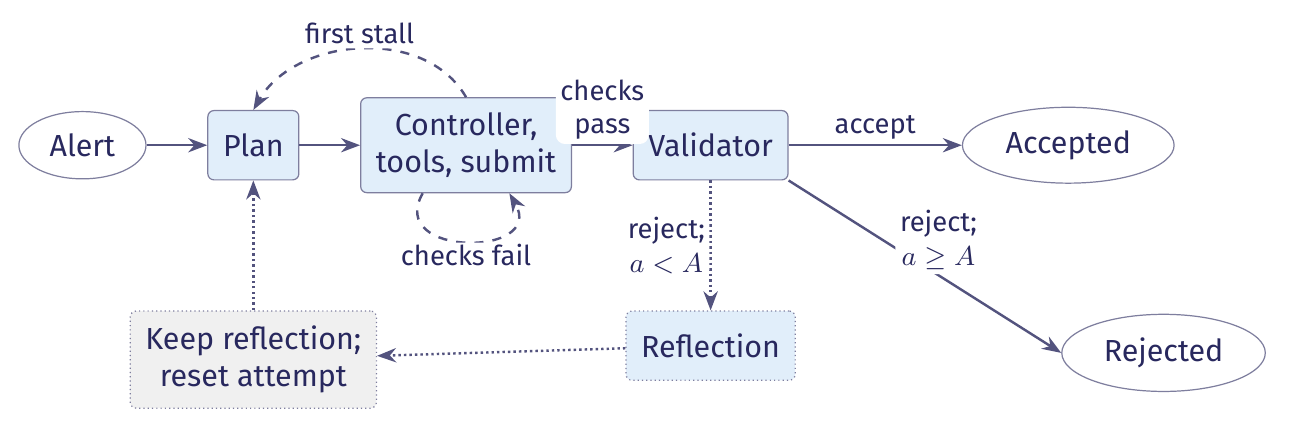
\includegraphics[width=0.78\textwidth]{figures/deck/81a0772b82.png}
  \caption{The proposed feedback edge for new attempts, from the validator back to the plan node.
  A rejection leads to a new attempt while $a$, the number of attempts so far, is below the attempt
  limit $A$, and ends the run otherwise.}
  \label{fig:routing-attempt}
\end{figure*}

After a rejection, the run either writes a reflection, resets the attempt and returns to
\demoref{plan}, or ends, depending on how many attempts it has made. We write $a$ for the value of the attempt
counter and $A$ for the attempt limit. When the validator rejects a patch and $a < A$, the run writes
a reflection and starts a new attempt. When $a \ge A$, the run ends with the status
\demoref{rejected}.

With the new attempt, the plan, the candidate patch and the check results would become attempt
fields, which hold the results of one attempt (\cref{sec:records}). The reset before a new attempt
clears them, so that no later step treats the rejected attempt's results as current. The reflection
survives the reset, and so do the run's counters.

The attempt counter must count attempts across the whole run. If each reset erased it, the counter
would read zero at the start of every attempt, and the runtime could not enforce a limit on the
total number of attempts. The counter therefore has run lifetime, like \demoref{model\_calls}. The
call budget still applies across all attempts.

Every feedback edge must have its own limit or rely on a limit for the whole run. Revision has its
own limit of one per run. Repair and the tool loop rely on the call budget, because both return to
the controller, which either ends the run or makes a model call. The proposed new attempt has both,
the attempt limit and the call budget.

\subsection{Loop bounds and termination}
\label{sec:routing-termination}

A condition for success does not guarantee that a run stops, so termination needs an argument of
its own. The argument answers the question Lecture~2 left open: when do the stopping rules guarantee
that a run ends?

An \textbf{acceptance predicate} is the condition under which a run is declared successful. In the
planning agent, a patch satisfies it when it passes the three submit checks and the validator
accepts it. The \textbf{acceptance procedure} is the code that evaluates the predicate: the submit
checks, followed by the validator's verdict.

A run that never produces an acceptable patch can keep cycling through its feedback edges unless
something else stops it. The acceptance predicate therefore says nothing about whether a run ends.

The usual argument uses a \textbf{loop variant}, a nonnegative integer that decreases on every
continuing cycle \citep{cornell-cs2112-loopinv}. A \textbf{continuing cycle} is one pass around a
loop of the graph, back to the location where it began, after which the run does not end. Because
the variant cannot fall below zero, it bounds the number of cycles. A variant that starts at $n$
allows at most $n$ continuing cycles.

In the planning agent, the variant is $B - c$: the call budget $B$ minus the number $c$ of calls
already made. With our budget of 40, it starts at 40. The argument rests on three conditions:
\bi
\item \textbf{Nonnegative.} The admission check (\cref{sec:records}) keeps $B - c$ nonnegative,
because a node makes a model call only while $c < B$.
\item \textbf{Decreasing.} Every continuing cycle makes at least one model call, so $B - c$ drops by
at least one per cycle.
\item \textbf{Each step returns.} Every step between two model calls returns or times out, so the run
reaches its next model call or its end.
\ei
Under these conditions, a run completes at most $B$ continuing cycles. The conditions bound the
number of cycles. They do not by themselves bound how long a single step takes.

The planning agent meets the decreasing condition. Every loop of its graph passes through the
controller, and a visit to the controller either ends the run or makes a model call. A cycle that
made no model call would leave $B - c$ unchanged, so the budget would not bound it. Such a cycle
needs its own limit. For example, a loop that only reruns tools or checks would need a counter of
its own.

The stall check does not provide a termination argument. It detects identical results. A run whose
tools keep returning different but irrelevant results, for example searches with different patterns
that each find unrelated lines, never triggers it. Such a run can continue without progress until the
budget ends it. Detecting one failure pattern does not prove termination. In our agent, the
termination argument rests on the call budget, provided that every step returns or times out.

Repetition has been observed in reactive agents. ReAct, short for reasoning and acting, is the
pattern that the reactive loop of Lecture~2 follows. In a manual analysis of sampled ReAct
trajectories on a question-answering task, one frequent error pattern was a model that generated its
previous thoughts and actions again and failed to leave the loop \citep[\S3.3]{yao2023react}. Our
stall check detects one consequence of such repetition, identical observations.

The call budget, the stall check and the recursion limit can each end a run before the validator
gives a verdict:
\bi
\item \textbf{The call budget.} Each node that calls a model, namely \demoref{plan},
\demoref{controller} and \demoref{validate}, runs the admission check before it calls the model
(\cref{sec:records}). When
\demoref{model\_calls} has reached the budget of 40, the node returns the status
\demoref{budget\_exhausted} instead of making the call. The check runs before the call, because a
check after the call would let the call incur its cost before the limit was enforced.
\item \textbf{The stall check.} The first stall triggers plan revision (\cref{sec:routing-feedback}).
A second stall, after the revision, ends the run with the status \demoref{no\_progress}.
\item \textbf{The recursion limit.} A \textbf{superstep} is one step of the graph runtime. The
\textbf{recursion limit} caps the number of supersteps in a single run \citep{langgraph-graph-api}.
In our agent it is four times the call budget. It counts supersteps without regard to the task or
to the cost of a step.
\ei

The budget and the recursion limit bound different quantities. The budget counts model calls, which
carry the run's cost. The recursion limit counts supersteps of every kind, so it would also end a
cycle that makes no model call. It would do so only after many supersteps, and it cannot distinguish
a useful step from a wasted one. A cycle without model calls therefore still needs a limit of its
own, tied to what the cycle does.

\subsection{What a trace establishes}
\label{sec:routing-trace}

A trace can establish that a run terminated and that its acceptance procedure passed. No trace event
can establish that the patch is correct. The following claims about a finished run must therefore be
kept apart:
\bi
\item \textbf{Execution stopped.} The \textbf{terminal event} is the event of kind
\demoref{terminal}. It is normally the trace's last event, and its \textbf{terminal status} states
how the run ended. A terminal event establishes that execution terminated.
\item \textbf{Acceptance passed.} A terminal event with the status \demoref{accepted} establishes
that the acceptance procedure passed. The patch passed the submit checks, and the validator accepted
it.
\item \textbf{The patch meets the postcondition.} In the specification of a method, the
\textbf{postcondition} is the implementer's obligation, a condition on the program's state after the
method runs \citep{mit6031-specs}. For a task, it is the condition that the finished artifact, here
the patch, must satisfy. No trace event establishes this claim.
\ei

For our patching task, the postcondition is what Lecture~2's performance measure asks: the weakness
is gone, and the endpoint still behaves as it did. The acceptance procedure produces evidence about
the patch. The submit checks show that the patch applies, touches the flagged line and leaves the
rescan clean.

A clean rescan shows only that the scanner no longer recognizes the flagged pattern (Lecture~2), and
none of the checks runs the endpoint. The validator adds a model's judgment of the patch. Passing
this procedure therefore does not prove that the patch satisfies the postcondition. The trace records
the outcome of the acceptance procedure. It does not establish that the patch is correct.

The model may propose that the work is finished, for example by replying without a tool call. The
submit checks, the validator and the limits then decide how the run ends, and the code of the nodes
sets the terminal status. The validator's verdict comes from a model, but the code of the
\demoref{validate} node turns it into the status \demoref{accepted} or \demoref{rejected}. No model
reply writes the status field directly.

A run of the planning agent ends with one of the following terminal statuses:
\bi
\item \textbf{\demoref{accepted}.} The validator accepted a patch that had passed the submit checks.
\item \textbf{\demoref{rejected}.} The validator rejected the patch.
\item \textbf{\demoref{budget\_exhausted}.} An admission check found the call budget spent before a
model call.
\item \textbf{\demoref{no\_progress}.} The run stalled again after its one plan revision.
\item \textbf{\demoref{error}.} An exception escaped the run.
\ei
The status \demoref{running} marks a run that is still active, so it is never a terminal status.

When a run ends normally, its trace must contain a terminal event. A run ends normally when it
reaches \demoref{END} without an exception. Every exit of the graph sets the status field, and the
runtime records that status in a terminal event before the trace is closed. The trace writer, the
code that appends events to the trace and closes it, checks this rule at closure. If no terminal
event has been written, closing the trace raises an exception that reports a run closed without
stating how it ended.

Every normal ending sets a status, so a terminal event missing at normal closure means that the
recording failed. Such a missing event is an \textbf{instrumentation defect}: a fault in the code
that records the run, which did not record how the run ended.

An escaped exception and a killed process leave different records. If an exception escapes the run,
the trace writer records a terminal event with the status \demoref{error}. It then writes a separate
\demoref{state\_change} event that names the exception, so in this case the terminal event is not
the last event. A
\demoref{SIGKILL} is the operating-system signal that ends a process immediately. The process cannot
intercept it, so none of its code runs after the signal, and no terminal event is written.

\Cref{tab:routing-trace} lists what a reader may conclude from each way a trace can end. The row that
needs the most care is the last one, a trace with no terminal event.

\begin{table}[htbp]
  \caption{What a trace records about the end of a run, and what that record supports.}
  \label{tab:routing-trace}
  \begin{adjustbox}{width=\linewidth}\begin{tabularx}{\linewidth}{L{0.36\linewidth}X}
    \toprule
    \textbf{What the trace records} & \textbf{What it supports} \\
    \midrule
    \textbf{A verdict, then a terminal event with status \demoref{accepted}} & Execution terminated
    and the acceptance procedure passed. The trace does not establish that the patch meets the
    task's postcondition. \\
    \addlinespace
    \textbf{A terminal event with status \demoref{rejected}, \demoref{budget\_exhausted},
    \demoref{no\_progress} or \demoref{error}} & Execution terminated without acceptance, for the
    reason the status states. The events before the ending record how far the run got. For
    \demoref{error}, the next event names the exception. \\
    \addlinespace
    \textbf{No terminal event} & The trace does not establish termination. The run may still be
    active, or the process may have been killed before it could write a terminal event. \\
    \bottomrule
  \end{tabularx}\end{adjustbox}
\end{table}

Labeling a run \demoref{error} because its trace has no terminal event assigns a cause without
evidence. The status \demoref{error} states that an exception escaped the run, and a trace without a
terminal event does not show that. The run may still be active, or it may have been killed. The
accurate reading is that the trace establishes neither whether the run ended nor how.

\subsection{A recorded repair and a keyboard interruption}
\label{sec:routing-recorded}

A second recorded run of the planning agent shows the repair edge taken twice and a run ended by an
interruption. The run worked on a path-traversal alert in OWASP BenchmarkPython, an alert about a
file path that may be built from outside input.

The first patch applied successfully. It left the flagged line unchanged, however, and the rescan
still reported the alert. The trace shows the following sequence:
\bi
\item \textbf{The checks.} The \demoref{submit} node recorded its check results: the patch applies,
it does not touch the flagged line, and the rescan is not clean. It also recorded a reason for each
failed check.
\item \textbf{The routing event.} The next event routed the run to the controller with
\demoref{by} set to \demoref{runtime}, because the tested value was a check result. It stated that
the submit checks had failed and listed both reasons.
\item \textbf{The repair.} The controller received both reasons as a conversation message. It then
ran further rounds through the tools (\cref{sec:machines}) and submitted again.
\ei

The second submission left the rescan clean, but the patch still did not touch the flagged line.
That check failed, the runtime returned its reason to the controller, and the repair edge was taken
a second time.

After more rounds through the tools, a keyboard interrupt stopped the run. A keyboard interrupt is
the signal sent when a user presses Ctrl-C, and Python raises it inside the program as the exception
\demoref{KeyboardInterrupt}. The trace ends with the last tool result, a terminal event with the
status \demoref{error}, and a \demoref{state\_change} event that names the exception. This ending falls in the second row of
\cref{tab:routing-trace}. The trace establishes that execution terminated without acceptance, and it
names the exception. It does not establish what the process was doing between the last tool result
and the interrupt.

A \demoref{SIGKILL} at the same point would have left a different trace. The trace would end at the
last tool result, with neither a terminal event nor the event that names an exception. It would fall in the last
row of \cref{tab:routing-trace}, and it would not establish that the run terminated.

Neither recorded run ended with the status \demoref{budget\_exhausted}. What we have said about that
ending is inferred from the transition rules. No recorded trace shows it.

\subsection*{Key points}
\bi
\item At each visit to a control location that has a routing function, the function tests the merged
record and selects one destination, so one compiled graph can send a run along different paths.
\item The \demoref{by} field of a routing event records whether the model or the runtime supplied the
tested value, and the programmer writes every guard in both cases.
\item For an active run, the routing function after the controller tests only whether the last reply
contains tool calls, so text in a reply that claims the work is finished has no effect on routing.
\item Every feedback edge needs a trigger, the information it passes back and a bound: revision is
limited to one per run, repair by the call budget, and the proposed new attempt by an attempt
counter that survives every reset and by the call budget.
\item An acceptance predicate only defines success, so termination needs a loop variant, here the
budget minus the calls made, which bounds only the cycles that make a model call, so a cycle without
one needs a limit of its own besides the recursion limit, which counts supersteps without regard to
the task, and the stall check, which detects one failure pattern, does not prove termination.
\item A terminal event establishes that a run terminated and the status \demoref{accepted}
establishes that the acceptance procedure passed, while no trace event establishes that the patch
meets the task's postcondition.
\item A trace without a terminal event does not establish termination, because the run may still be
active or its process may have been killed, so labeling such a run \demoref{error} assigns a cause
without evidence.
\ei

\section{Vulnerability management and discovery (the HW1 domain)}
\label{sec:discovery}

The planning agent of the first three sections (\cref{sec:machines,sec:records,sec:routing})
receives one scanner alert and patches it without asking whether the alert points to a flaw that an
attacker could use. The first homework, HW1, asks an agent to answer that question for every alert,
and designing such an agent requires a precise statement of the task. This section places the task
within vulnerability management, describes how discovery tools produce alerts, and introduces what
is needed to judge an alert: the attack surface, the threat model and the catalogues that classify
flaws. \Cref{sec:triage} then turns to Bandit's alerts and to triage itself.

\subsection{Vulnerability management and its stages}
\label{sec:discovery-stages}

\textbf{Vulnerability management} is the work of finding the flaws in a program that an attacker
could use, deciding which of them are real, proving that they are real, and fixing them. We use the
plain word \emph{flaw} for a defect of this kind. \Cref{sec:triage} defines the more precise term
\emph{vulnerability}.

The work has four stages, and each stage takes the result of the one before it:
\bi
\item \textbf{Discovery.} Discovery turns a repository and a scope, the part of the code to be
examined, into alerts. As in Lecture~2, an alert is a report that names a file, a line and the kind
of flaw suspected there.
\item \textbf{Triage.} Triage turns each alert into a label, together with the evidence for it. A
\textbf{label} is the verdict on one alert. In HW1 it is 1 when an attacker, as the threat model
defines one (\cref{sec:discovery-threat}), can reach the flaw the alert points to, and 0 when no
such attacker can.
\item \textbf{Validation.} Validation proves that a flaw kept by triage is real by reproducing it,
for example by running the program on an input that makes the flaw occur.
\item \textbf{Patching.} Patching changes the code so that a proven flaw is gone and the program
still behaves as it did for legitimate use.
\ei

The stages narrow the work step by step. Discovery may report many alerts, triage keeps the ones an
attacker can reach, validation confirms them, and patching removes them. A mistake in one stage
carries into the next. An alert that triage wrongly keeps costs work later, and a real flaw that
triage wrongly drops is never patched.

HW1 builds the first two stages. Its discovery stage is a fixed scan with one tool
(\cref{sec:discovery-alerts}), and the agent you build in HW1 performs triage. Validation and
patching come later in the course, with HW2 and HW3.

The planning agent works at the last of these stages, patching. HW1 adds the triage stage that the
planning agent skips.

Validation in this sense names a stage of vulnerability management. It is distinct from the planning
agent's validator (Lecture~2, Section~4), which judges whether a submitted patch should be accepted.

\subsection{Kinds of discovery tool}
\label{sec:discovery-tools}

Tools discover flaws in different ways, and each way misses some flaws. A discovery tool reads the
program's code, runs the program and watches how it behaves, or checks the libraries that the
program depends on. Static application security testing (\textbf{SAST}) reads the code. Dynamic
application security testing (\textbf{DAST}) and \textbf{fuzzing} run the program, and
\textbf{dependency scanning} checks its libraries. \Cref{tab:discovery-tools} summarizes how each
kind finds flaws, and the list after it gives what each kind misses.

\begin{table}[htbp]
  \caption{Kinds of discovery tool and how each one finds flaws.}
  \label{tab:discovery-tools}
  \begin{adjustbox}{width=\linewidth}\begin{tabularx}{\linewidth}{L{0.3\linewidth}X}
    \toprule
    \textbf{Kind} & \textbf{How it finds flaws} \\
    \midrule
    \textbf{SAST} & Matches rules against the source code, without running the program \\
    \textbf{DAST} & Runs the program and attacks it from outside, watching how it responds \\
    \textbf{Fuzzing} & Feeds the program generated inputs and keeps the inputs that make it crash \\
    \textbf{Dependency scanning} & Checks the program's libraries against published records of flaws \\
    \bottomrule
  \end{tabularx}\end{adjustbox}
\end{table}

Each kind sees some flaws and misses others:
\bi
\item \textbf{SAST.} A SAST tool reads the code without running it. Lecture~2 called a tool of this
kind a static-analysis scanner. It can examine every line, including code that no test reaches. It
never sees the values that arrive while the program runs, so where a value comes from must be
inferred from the code. Bandit's rules make no such inference, because each one matches only the
shape of the code (\cref{sec:triage}).
\item \textbf{DAST.} A DAST tool runs the program, sends it requests from outside, as an attacker
would, and watches its responses. It finds only flaws in the code that its requests cause to run.
\item \textbf{Fuzzing.} Fuzzing is dynamic testing in which the inputs are generated
automatically instead of crafted by hand. The tool keeps the inputs that make the program crash.
Like DAST, it finds only flaws in the code that its inputs cause to run.
\item \textbf{Dependency scanning.} Dependency scanning, also called software composition analysis,
compares the libraries a program uses, and their versions, with published records of known flaws.
It finds only flaws that are already known in those libraries. Flaws in the program's own code are
outside its view.
\ei

HW1 discovers flaws with one SAST tool, Bandit, a static-analysis scanner for Python, which also
produced the worked alert of Lecture~2 \citep{bandit}. HW2 and HW3 add other kinds of discovery
tool.

\subsection{Rules and what they match}
\label{sec:discovery-rules}

A SAST tool finds flaws with rules. A \textbf{rule} consists of a pattern, which is the shape of
code to look for, a message to print when the pattern matches, and metadata that classifies the
match.

% Defined here, ahead of the text that discusses it, so that this two-column float reaches the top
% of the next page, where that text runs.
\begin{figure*}[t]
  \centering
  \begin{adjustbox}{max width=\textwidth}
  \begin{tikzpicture}[
    card/.style={draw=ibmfg!60, rounded corners=2pt, fill=white, inner sep=5pt, align=left,
                 font=\sffamily\small},
    note/.style={font=\sffamily\footnotesize, text=black!60, align=center},
    bind/.style={-{Stealth[length=2mm]}, thick, draw=ibmblue},
    emit/.style={-{Stealth[length=2mm]}, thick, draw=ibmfg!80, rounded corners=3pt},
  ]
    \node[card, text width=58mm] (rule) at (0,0) {%
      \textbf{bandit.B608}, the port of Bandit's rule\\[3pt]
      \texttt{pattern-inside:}\\
      \texttt{\ \ \textcolor{ibmblue}{\$SQL} = f"...\{\textcolor{ibmblue}{\$X}\}..."}\\
      \texttt{pattern:}\\
      \texttt{\ \ \textcolor{ibmblue}{\$DB}.execute(\textcolor{ibmblue}{\$SQL})}\\[3pt]
      cwe: CWE-89\quad owasp: A1: Injection};
    \node[note, above=1mm of rule] {the rule: a pattern with gaps};
    \node[card, text width=88mm, anchor=north west] (code) at ($(rule.north east)+(24mm,0)$) {%
      \textbf{BenchmarkTest00099}\\[3pt]
      \texttt{\textcolor{black!50}{46} \textcolor{ibmblue}{sql} = f\textquotesingle SELECT username from USERS}\\
      \texttt{\phantom{46} where password = \textbackslash\textquotesingle\{\textcolor{ibmblue}{bar}\}\textbackslash\textquotesingle\textquotesingle}\\
      \texttt{\textcolor{black!50}{49} \textcolor{ibmblue}{cur}.execute(\textcolor{ibmblue}{sql})}};
    \node[note, above=1mm of code] {the code that fills the gaps};
    \node[note, below=1mm of code] (binding)
      {\texttt{\$SQL} = \texttt{sql},\quad \texttt{\$X} = \texttt{bar},\quad \texttt{\$DB} = \texttt{cur}};
    \node[card, text width=78mm, anchor=north] (alert) at ($(rule.south)+(18mm,-15mm)$) {%
      \textbf{alert}\quad bandit.B608 at line 49\\
      CWE-89 SQL injection, A1: Injection, severity WARNING};
    \node[note, below=1mm of alert] {the alert, with its kind and family of flaw attached};
    \draw[bind] (rule.east |- code.west) -- node[note, above] {binds} (code.west);
    \draw[emit] (binding.south) |- node[note, pos=0.3, right] {matches} (alert.east);
  \end{tikzpicture}
  \end{adjustbox}
  \caption{A Semgrep rule matching a BenchmarkPython test case. The metavariables of GitLab's port of
  Bandit's rule B608 bind to the variables of lines 46 and 49, and the match is reported as an alert
  that carries the rule's CWE number and Top 10 family.}
  \label{fig:discovery-binding}
\end{figure*}

Bandit's own rules are part of its Python source code (\cref{sec:triage}). Semgrep is another SAST
tool, whose rules are written as short text files, so the parts of a rule can be read directly
\citep{semgrep-rule-syntax}. GitLab has rewritten Bandit's rules in Semgrep's format
\citep{gitlab-semgrep-bandit}. A rule rewritten for another tool is called a port.

A Semgrep pattern is a piece of code with gaps in it. A gap is written as a \textbf{metavariable}, a
name that begins with \texttt{\$} and contains only capital letters, digits and underscores, such as
\texttt{\$X}. A metavariable matches one element of code in its position, such as a variable, an
expression or the name of a function. Three dots, called an ellipsis, match a sequence of zero or
more items: the arguments of a call, statements, or the characters inside a string.

When a pattern matches, each metavariable is bound to the code that fills its gap, and the tool
reports an alert at the matched line. Semgrep calls an alert a finding.

\Cref{lst:discovery-b610} shows the port of Bandit's rule B610, with two of its three patterns and
the end of its message left out.

\begin{lstlisting}[basicstyle=\ttfamily\footnotesize, caption={Bandit's rule B610 as GitLab ported it to Semgrep, shortened.}, label=lst:discovery-b610]
- id: bandit.B610
  patterns:
  - pattern-either:
    - pattern: $X.objects.$FUNC(...).extra(...)
    # two longer patterns omitted
  message: This is a last resort. You should be careful when using QuerySet.extra due to SQLi ...
  metadata:
    cwe: "CWE-89: Improper Neutralization of Special Elements used in an SQL Command ('SQL Injection')"
    owasp: 'A1: Injection'
  severity: ERROR
  languages: [python]
\end{lstlisting}

The rule has the following parts:
\bi
\item \textbf{Identifier.} The field \texttt{id} names the rule after the Bandit rule it ports.
\item \textbf{Pattern.} The block \texttt{patterns} gives the shape of code to match, and
\texttt{pattern-either} means that any one of the listed patterns may match. This pattern matches a
call to \texttt{extra} at the end of a database query written with Django, a Python web framework.
In it, \texttt{\$X} and \texttt{\$FUNC} stand for any class and any method, and the dots stand for
any arguments. The method \texttt{extra} lets a query include raw SQL text.
\item \textbf{Message.} The field \texttt{message} is the text the tool prints with each match. Here
it warns that \texttt{extra} can lead to SQL injection.
\item \textbf{Metadata.} The field \texttt{cwe} gives the kind of flaw by its number in the Common
Weakness Enumeration, a public catalogue of kinds of flaw. In this rule it is CWE-89, SQL
injection. The field \texttt{owasp} names the flaw's family: the entry of the OWASP Top 10, a second
public list, to which the flaw belongs. \Cref{sec:discovery-top10,sec:discovery-cwe} describe both
lists.
\item \textbf{Severity and language.} The field \texttt{severity} is the rule's estimate of the harm
if a match is a real flaw. Semgrep grades it with words such as ERROR and WARNING, and Bandit grades
it as LOW, MEDIUM or HIGH (\cref{sec:triage}). The field \texttt{languages} names the programming
languages whose files the rule applies to.
\ei
A rule therefore carries the shape to match, the message to print, and the kind and family of flaw
that a match belongs to.

\Cref{fig:discovery-binding} shows a rule binding to real code. The rule is GitLab's port of
Bandit's B608, which looks for SQL queries built from strings. Its \texttt{pattern-inside} clause
requires that the match lie inside code where a variable \texttt{\$SQL} is assigned an f-string with
a gap \texttt{\{\$X\}}. Inside the string, the dots match any characters, so the clause accepts any
f-string with a gap. Its \texttt{pattern} clause then requires a call \texttt{\$DB.execute(\$SQL)}
with that variable as its only argument.

The code is the test case BenchmarkTest00099 of OWASP BenchmarkPython, the Python web application
that the planning agent works on (\cref{sec:machines}). As in Lecture~2, a test case is a short program
that handles one kind of web request. Line~46 builds a query as an f-string with \texttt{bar} in
its gap, and line~49 executes it. The names set in blue are the metavariables and the code they
bind to: \texttt{\$SQL}~=~\texttt{sql}, \texttt{\$X}~=~\texttt{bar} and \texttt{\$DB}~=~\texttt{cur}.
The port reports an alert at line~49 with CWE-89, the family tag A1: Injection, and the severity
this rule assigns, WARNING.

A rule can hold several patterns, one for each way of writing the same flaw. Besides the form of
\cref{fig:discovery-binding}, the port's B608 entry matches a query built with the \texttt{\%}
operator, with \texttt{.format}, with an f-string or by concatenation directly inside the call to
\texttt{execute}. It also matches a query built earlier with \texttt{\%} or \texttt{.format} and
stored in a variable.

Which code produces an alert depends only on the rule's pattern. GitLab's port writes the pattern
of B608 in Semgrep's notation, while Bandit's own B608 is Python code that checks whether the text
of a string looks like a SQL query (\cref{sec:triage}). The two patterns differ, so the two
implementations report different alerts:
\bi
\item \textbf{The reported line.} Bandit's own B608 reports the flaw of
\cref{fig:discovery-binding} at line~46, where the query is built. The port reports line~49, where
the query is executed.
\item \textbf{The matched code.} Another test case, BenchmarkTest00011, writes its query as an
f-string with no gap and passes the value to the database separately, as a bound parameter
(Lecture~2). The port does not match it. Its query has no gap for \texttt{\$X} to bind, and its
call to \texttt{execute} passes a second argument, which \texttt{\$DB.execute(\$SQL)} does not
allow. Bandit's own B608 does report it, because it flags any f-string whose text looks like a SQL
query, whether or not the f-string has a gap.
\ei

\subsection{What an alert contains}
\label{sec:discovery-alerts}

In HW1, discovery runs Bandit's fixed set of rules over the code and reports every place where a
rule matches. Each alert names a file, a line, the rule that matched and the kind of flaw that the
rule suspects, so that the next stage knows where to look. An alert records only that a rule
matched. Whether the match is a real flaw is left open, and deciding it is the job of triage.

The worked alert of Lecture~2 is an example. Bandit's rule B608 matched a line of BenchmarkPython that
builds a SQL query by interpolation, and the alert named the file, that line and the rule. The alert
did not say whether a value supplied by a user could reach the query. BenchmarkTest00099, the test
case of \cref{fig:discovery-binding}, is a different test case. It builds and runs its query with the
same two lines as the worked alert's test case, at lines~46 and~49, and Bandit reports it in the
same way, at line~46.

HW1 scans three targets with Bandit 1.9.4 and keeps the alerts that Bandit rates at MEDIUM severity
or higher. The three targets are the following:
\bi
\item \textbf{OWASP BenchmarkPython.} The first 99 test cases of BenchmarkPython give 18 alerts
\citep{owasp-benchmarkpython}.
\item \textbf{Radicale.} Radicale, a calendar server, gives 10 alerts \citep{radicale}.
\item \textbf{SGLang.} SGLang, a server that runs large language models and answers requests to
them, gives 21 alerts \citep{sglang}.
\ei

Each target is pinned at one commit, a fixed version of its code, and Bandit's rules are fixed as
well. Scanning the same commit therefore gives the same list of alerts every time. Every agent built
for HW1 receives the same alerts, and two runs of an agent can be compared alert by alert.

The targets play different roles in HW1. BenchmarkPython ships an \textbf{answer key}, a file that
records the true labels: for each test case, its category, the CWE number it tests, and whether its
flaw is real. A \textbf{development set} is a target whose answer key is open to students, so that
they can check their agent's labels while they build it. The first 99 test cases of BenchmarkPython
are HW1's development set.

The agent itself never reads the answer key (Lecture~2, Section~2). An agent that could read it would
copy its labels instead of analyzing the code. A \textbf{held-out target} is a target whose answer
key stays hidden. Radicale and SGLang are held out, so they measure how the agent performs on code
it was not tuned on.

\subsection{The attack surface}
\label{sec:discovery-surface}

An attacker can affect a program only through the data the program takes in from outside. That data
arrives at a few places, such as a request, a file or a message, and an attacker starts there. The
\textbf{attack surface} of a program is the set of places where data from outside the program enters
it, together with the code that first handles that data.

\begin{definition}[Attack surface]
\label{def:discovery-surface}
``Intuitively, a system's attack surface is the set of ways in which an adversary can enter the
system and potentially cause damage.'' \citep[\S1]{manadhata2007approach}
\end{definition}

In the formal version of this definition, a system's attack surface consists of its entry and exit
points, its channels and its untrusted data items \citep{manadhata2011attack}. For triage, the part
that matters most is where data enters. An \textbf{entry point} is one place where data from outside
enters the program.

Each HW1 target has its own attack surface:
\bi
\item \textbf{BenchmarkPython.} Every test case is a Flask route, a function that the Flask web
framework calls to handle requests to one address, and it reads a cookie or a form field from the
request. Its surface is the request.
\item \textbf{Radicale.} Radicale is a calendar server, so its surface is the HTTP request that a
client sends, whether the client has logged in or not.
\item \textbf{SGLang.} SGLang is a server for large language models. Its surface includes the
request, and also the model files it loads and the channels over which its own worker processes
exchange messages.
\ei

\Cref{lst:discovery-entry} shows one entry point in code, the start of the test case of
\cref{fig:discovery-binding}.

\begin{lstlisting}[basicstyle=\ttfamily\footnotesize, caption={The entry point of the test case BenchmarkTest00099 and the path of its value to \texttt{bar} (lines 31 to 42, with lines 34 to 37 and 40 left out).}, label=lst:discovery-entry]
31  param = request.form.get("BenchmarkTest00099")
32  if not param:
33      param = ""
38  conf52528 = configparser.ConfigParser()
39  conf52528.add_section('section52528')
41  conf52528.set('section52528', 'keyB-52528', param)
42  bar = conf52528.get('section52528', 'keyB-52528')
\end{lstlisting}

Line~31 is the entry point. It reads a form field of the incoming request, and the client who sends
the request controls its value. Lines~32 and~33 replace a missing value with an empty string.
Lines~38 to~42 store the value in a configuration object under one key and read it back under the
same key, so \texttt{bar} holds exactly what the client sent. This detour is the benchmark's way of
hiding a flow of data from a scanner.

A \textbf{sink} is the call where outside data can do harm, such as the call that sends a query to a
database. In BenchmarkTest00099, line~46 places \texttt{bar} in the query text, and line~49 sends
that text to the database (\cref{fig:discovery-binding}). Line~49 is the sink, and whatever the
client sends in the form field is the value of \texttt{bar} there. A scanner's rule usually points
at the sink or at the line that prepares its argument. GitLab's port points at line~49, and
Bandit's own B608 points at line~46 (\cref{sec:discovery-rules}).

For every alert, the agent you build in HW1 asks whether the value at the flagged line can come from
the attack surface. In this test case it can. The value read at line~31 reaches the sink at line~49
unchanged.

\subsection{The threat model}
\label{sec:discovery-threat}

A label says whether an attacker can reach a flaw, so it needs a definite attacker: who the attacker
is and which data they control. A \textbf{threat model} names the attacker, the data the attacker
controls, and the harm the attacker must be unable to do. \Cref{tab:discovery-threat} gives the
attacker of each HW1 target. Its last column, what the attacker controls, is what a label depends on.

\begin{table}[htbp]
  \caption{The attacker of each HW1 target and the data that attacker controls.}
  \label{tab:discovery-threat}
  \begin{adjustbox}{width=\linewidth}\begin{tabularx}{\linewidth}{L{0.22\linewidth}L{0.3\linewidth}X}
    \toprule
    \textbf{Target} & \textbf{The attacker} & \textbf{What they control} \\
    \midrule
    \textbf{Benchmark\-Python} & An anonymous web client & Every byte of the request: cookies, form fields, headers \\
    \textbf{Radicale} & A calendar client, logged in or not & The request, plus the storage directory if local users count \\
    \textbf{SGLang} & A client, or whoever publishes a model & The request, the model files it loads, and its worker channel \\
    \bottomrule
  \end{tabularx}\end{adjustbox}
\end{table}

% Defined in the threat-model subsection, ahead of the Top 10 text that first cites it, so that this
% two-column float reaches the top of the page on which that text runs (a table* defined on one page
% appears at the earliest on the next). It precedes the Top 10 table in the source because LaTeX keeps
% tables in number order: defined after it, it waits behind that table when the table is deferred.
\begin{table*}[t]
  \caption{From a Top 10 family to a CWE, to the Python call that carries the flaw, and to the
  BenchmarkPython category that tests it. The CWE numbers are those of the benchmark's answer key.}
  \label{tab:discovery-hierarchy}
  \begin{adjustbox}{width=\linewidth}\begin{tabularx}{\linewidth}{L{0.36\linewidth}L{0.08\linewidth}XL{0.15\linewidth}}
    \toprule
    \textbf{Family} & \textbf{CWE} & \textbf{The Python call} & \textbf{Benchmark category} \\
    \midrule
    \textbf{Injection} & CWE-89 & A query built from a string & \texttt{sqli} \\
    \textbf{Injection} & CWE-78 & A shell command built from a string & \texttt{cmdi} \\
    \textbf{Injection} & CWE-94 & \texttt{exec} or \texttt{eval} on a string & \texttt{codeinj} \\
    \textbf{Cryptographic Failures} & CWE-328 & MD5 or SHA1 applied to a secret & \texttt{hash} \\
    \textbf{Software or Data Integrity Failures} & CWE-502 & \texttt{pickle.load} or \texttt{torch.load} & \texttt{deserialization} \\
    \textbf{Security Misconfiguration} & CWE-611 & An XML parser applied to outside data & \texttt{xxe} \\
    \textbf{Broken Access Control} & CWE-22 & \texttt{open}, or a test that a file exists, on a path from outside & \texttt{pathtraver} \\
    \bottomrule
  \end{tabularx}\end{adjustbox}
\end{table*}

For BenchmarkPython the threat model is simple, because an anonymous client controls the whole
request. For Radicale and SGLang, the labels of most alerts depend on which attackers the threat
model counts:
\bi
\item \textbf{Radicale.} Seven of its ten alerts load files with Python's \texttt{pickle} module,
which turns stored bytes back into Python objects and can run code chosen by whoever wrote the file.
Radicale wrote these files itself, in its storage directory. The storage directory is in the
attacker's control only if the threat model counts local users of the machine as attackers.
\item \textbf{SGLang.} Eighteen of its 21 alerts load models, from model files or from the Hugging
Face Hub, or unpickle bytes that do not come from the HTTP request: pickled files on disk, and
messages on the channels over which SGLang's processes and their clients exchange work. Whether
they are reachable depends on whether the threat model counts as an attacker whoever publishes a
model, whoever writes those files, or whoever can send messages on those channels.
\ei

The labels of these alerts turn entirely on the threat model. Bandit ignores the threat model,
because its rules match the shape of the code and carry no information about who controls the data.

A \textbf{rationale} is the text that justifies a label. The agent you build in HW1 should state the
threat model once in its prompt, so that every label is decided under the same assumption. It should
state it again in every rationale, so that a reviewer can see which attacker the label assumed.
Without a stated threat model a label cannot be checked, because the same alert can deserve 1 under
one threat model and 0 under another.

\subsection{The OWASP Top 10}
\label{sec:discovery-top10}

The \textbf{OWASP Top 10} is a ranked list of the most critical security risks to web
applications, published by the OWASP Foundation (Open Worldwide Application Security Project). A
\textbf{family} is one of its ten entries: a group of related kinds of flaw, such as injection. The
current edition, the OWASP Top 10:2025, was announced as a release candidate on 6 November 2025 and
published in final form in December 2025 \citep{owasp2025top10}.
Eight of its families were chosen and ranked from data on over 2.8 million applications, and two
were added from a survey of practitioners. The analysis considered 589 kinds of flaw from the
catalogue described in \cref{sec:discovery-cwe}.

\Cref{tab:discovery-top10} lists the ten families with a plain description of each. The families
that matter most for HW1 are Software or Data Integrity Failures, Injection, Cryptographic Failures
and Security Misconfiguration. \Cref{tab:discovery-hierarchy} follows these families down to the
Python calls that carry their flaws, and \cref{sec:discovery-python} explains it.

\begin{table}[htbp]
  \caption{The ten families of the OWASP Top 10:2025, each with a plain description.}
  \label{tab:discovery-top10}
  \begin{adjustbox}{width=\linewidth}\begin{tabularx}{\linewidth}{>{\RaggedRight\arraybackslash\hyphenpenalty=10000\exhyphenpenalty=10000}p{0.56\linewidth}X}
    \toprule
    \textbf{Family} & \textbf{What goes wrong} \\
    \midrule
    \textbf{A01 Broken Access Control} & A user reaches data or actions that should be denied to them \\
    \textbf{A02 Security Misconfiguration} & A setting enables something that should be off \\
    \textbf{A03 Software Supply Chain Failures} & A dependency brings in unchecked code \\
    \textbf{A04 Cryptographic Failures} & Protection is missing or weak \\
    \textbf{A05 Injection} & Outside data becomes part of a command \\
    \textbf{A06 Insecure Design} & The design lacks a control it needed \\
    \textbf{A07 Authentication Failures} & The program fails to confirm who the user is \\
    \textbf{A08 Software or Data Integrity Failures} & Code or data is trusted without a check \\
    \textbf{A09 Security Logging and Alerting Failures} & An attack is not recorded, or its record is not reviewed \\
    \textbf{A10 Mishandling of Exceptional Conditions} & An error is handled in a way that grants access or reveals data \\
    \bottomrule
  \end{tabularx}\end{adjustbox}
\end{table}

The edition matters when reading a rule's metadata. The tag \texttt{A1: Injection} of
\cref{lst:discovery-b610} uses the numbering of the 2017 edition \citep{owasp2017top10}. In the 2025
edition, Injection is A05.

The 49 alerts of HW1 fall into the families as follows:
\bi
\item \textbf{Software or Data Integrity Failures.} This family has 26 alerts. They load pickled
data or model files, or download models without an integrity check.
\item \textbf{Injection.} This family has 7 alerts. They build SQL queries from strings, run
\texttt{exec} or \texttt{eval}, or start a shell command.
\item \textbf{Cryptographic Failures.} This family has 6 alerts, which use the MD5 or SHA1 hash.
\item \textbf{Security Misconfiguration.} This family has 6 alerts, which parse XML.
\Cref{sec:discovery-python} explains why XML parsing belongs to this family.
\item \textbf{None of the ten.} The remaining 4 alerts come from Bandit's rule B113, which no family
covers (\cref{sec:discovery-python}).
\ei
The integrity alerts of Radicale and SGLang are exactly the alerts whose labels turn on the threat
model (\cref{sec:discovery-threat}). The other integrity alert comes from BenchmarkPython.

\subsection{Weaknesses and their catalogues}
\label{sec:discovery-cwe}

A \textbf{weakness} is a kind of flaw that recurs across programs. Each family of the Top 10 is a
set of weaknesses from a public catalogue. The Common Weakness Enumeration (\textbf{CWE}) is that
catalogue, kept by MITRE, and it gives each weakness a number and a name \citep{mitre-cwe}. An entry
of the catalogue is also called a CWE. CWE-89, for example, is SQL injection, and it can occur in
any program, in any language, that builds a query from text.

CWE, CVE and CVSS are easily confused, because they describe flaws at different levels:
\bi
\item \textbf{CWE.} A CWE is a weakness, such as CWE-89. It describes no particular program.
\item \textbf{CVE.} A Common Vulnerabilities and Exposures record (CVE) identifies one
instance of a flaw in one product \citep{cve-program}. Its record usually names a CWE as the type
of the flaw.
\item \textbf{CVSS.} The Common Vulnerability Scoring System (CVSS) rates one instance of a
flaw by how easily an attacker can use it and how much damage it does
\citep{first2023cvss4}. A CVSS score therefore attaches to a CVE.
\ei

A family groups many CWEs. In the 2025 edition, the Injection family alone contains 37 CWEs,
including CWE-89 (SQL injection), CWE-78 (OS command injection), CWE-94 (code injection) and
CWE-95 (eval injection) \citep{owasp2025top10}.

Every HW1 alert carries a CWE number, because Bandit 1.9.4 attaches one to every alert it reports.
The number names the kind of flaw that the rule suspects at the flagged line.

\subsection{From a family to a line of Python}
\label{sec:discovery-python}

The Top 10 and the CWE catalogue form a hierarchy that continues into the code: a family contains
CWEs, and each CWE appears in code as a particular kind of Python call.
\Cref{tab:discovery-hierarchy} follows this hierarchy for several kinds of flaw that
BenchmarkPython tests. Its last column names the benchmark category whose test cases cover each
kind. The answer key has further categories, such as XPath injection (\cref{sec:triage}). Read each
row from left to right, from the general family to the specific call.

The call at the bottom of the hierarchy is the sink (\cref{sec:discovery-surface}). An alert's CWE
therefore usually tells the agent the family of the suspected flaw and the shape of code to look
for around the flagged line.

The CWE numbers in \cref{tab:discovery-hierarchy} are those of BenchmarkPython's answer key. Bandit
attaches its own numbers, which sometimes differ from the key:
\bi
\item \textbf{exec and eval.} Bandit reports CWE-78, OS command injection, where the key has CWE-94,
code injection. Both are Injection CWEs.
\item \textbf{MD5 and SHA1.} Bandit reports CWE-327, a broken or risky cryptographic algorithm, where
the key has CWE-328, a weak hash. Both belong to Cryptographic Failures.
\item \textbf{XML parsers.} Bandit reports CWE-20, improper input validation. The flaw these rules
look for is an XML external entity (XXE) flaw, in which an XML document makes the parser read a file
or contact a server that the document names. The key gives CWE-611 for its XXE cases. CWE-20 is an
Injection CWE in the 2025 edition, while CWE-611 belongs to Security Misconfiguration.
\ei

The XML alerts are the exception to this correspondence. Their CWE points to Injection, while the
flaw they look for belongs to Security Misconfiguration, which is where the counts of
\cref{sec:discovery-top10} place them. In the development set, the two XML alerts of
BenchmarkTest00017 fall in a test case of the XXE category. The XML alerts of BenchmarkTest00013 to
BenchmarkTest00016 fall in test cases of the XPath-injection category, for which the key gives
CWE-643 (\cref{sec:triage}).

A scanner's rules and the families of the Top 10 are separate lists. A rule can report a flaw that
no family contains, and a family can contain flaws that no rule reports. Bandit's rule B113 reports
an HTTP request made without a timeout, which can leave the program waiting indefinitely, and it
attaches CWE-400, uncontrolled resource consumption. CWE-400 belongs to none of the ten families,
so the four B113 alerts of HW1 have no family.

Path traversal is a flaw of the second kind. In a path traversal (CWE-22, Broken Access Control), a
request makes the program open a file outside the folder it intended. BenchmarkPython's
path-traversal cases open a file, or test whether a file exists, on a path built from the request,
and Bandit has no rule for either shape of code. The
path-traversal cases of the development set therefore receive no Bandit alert (\cref{sec:triage}).
The path-traversal alert of the second recorded run in \cref{sec:routing} came from a different
scanner.

\subsection*{Key points}
\bi
\item Vulnerability management has four stages: discovery turns code into alerts, triage turns each
alert into a label with its evidence, validation proves a kept flaw by reproducing it, and patching
removes a proven flaw while keeping the program's behavior.
\item Discovery tools read the code (SAST), run the program (DAST and fuzzing) or check its libraries
(dependency scanning), and a SAST tool such as Bandit matches rules, each made of a pattern, a
message and metadata.
\item An alert records only that a rule matched, and HW1's alerts come from one fixed Bandit scan of
a development set with an open answer key (BenchmarkPython's first 99 test cases) and of two
held-out targets (Radicale and SGLang).
\item The attack surface is the set of places where outside data enters a program, with the code
that first handles it, and triage asks whether the value at the sink can come from an entry point.
\item A threat model names the attacker, the data the attacker controls and the harm to prevent, and
because the same alert can deserve 1 under one threat model and 0 under another, the agent states it
in its prompt and in every rationale.
\item The OWASP Top 10:2025 ranks the most critical security risks to web applications as ten
families, each a set of CWEs, where a CWE is a kind of flaw, a CVE is one instance of a flaw in one
product, and a CVSS score rates that instance.
\item An alert's CWE usually names its family and the shape of code to look for, although Bandit's
XML alerts point to the wrong family and the B113 alerts belong to no family.
\ei

\section{Bandit alerts and triage}
\label{sec:triage}

\Cref{sec:discovery} named the weaknesses that HW1's alerts point to and the attacker against whom
each one matters. This section describes the alerts themselves, which are what the agent you build in
HW1 receives and must label. We show how Bandit reads a program, what its rules and alert records
contain, and when a matched weakness is a vulnerability, using alerts from the development set with
and without a real flaw behind them. We then explain why every alert needs triage, what each kind of
triage mistake costs, how alerts are prioritized, and what a label must carry.

\subsection{How Bandit reads a program}
\label{sec:triage-tree}

Bandit finds alerts by matching shapes in the structure of a program, without running it. A
\textbf{syntax tree} is the tree that a parser builds from source code. Each node stands for one
construct of the language, such as an assignment, a function call or a name, and the children of a
node are the parts of that construct. Bandit parses each Python file into the syntax tree that
Python's own parser produces \citep{python-ast} and runs every rule against the nodes of the tree
\citep{bandit}.

A rule, as \cref{sec:discovery} defined it, is a pattern, a message and metadata. In Bandit, the
pattern is a shape in the syntax tree, for example a call to a function with a given name. When a
node has that shape, the rule reports an alert at the line where the node occurs, together with the
rule's message and its severity (\cref{sec:triage-severity}).

What a rule can see is limited to the part of the tree it reads. A rule reads the node it matched and
a few nodes near it, which record the call as it is written: which function is called and what is
passed to it. The rule does not follow a name back through the assignments that gave the name its
value. It therefore learns nothing about where an argument's value came from. When the argument is a
variable, as \texttt{fb} is in \cref{fig:triage-tree}, the rule cannot tell whether the variable holds
a value read from a request or a constant assigned a few lines earlier.

Every Bandit alert reports a matched shape and leaves open where the data at that shape comes from.
Whether data from an attacker can reach the matched call is the question that triage answers
(\cref{sec:triage-undecided}).

\begin{figure*}[t]
  \centering
  \begin{adjustbox}{width=\textwidth}% One Bandit match, in three panels: one line of Radicale, its syntax tree, and the name list of
% rule B301. The highlighted path is what the rule reads: the called name, pickle.load. The
% argument fb is a leaf the rule never visits. Redrawn for the notes from
% lecture-3--2026-09-25/slides/figures/hw1-ast-rule.tikz (lecture3-hw.pptx slide 21), without the
% file-path labels. Styles are local so the figure needs nothing beyond the notes' preamble.
\begin{tikzpicture}[
  tn/.style={gnode, font=\sffamily\small, minimum height=7mm, inner sep=4pt},
  card/.style={draw=ibmfg!60, rounded corners=3pt, fill=white, inner sep=6pt, align=left,
               font=\sffamily\small},
  hl/.style={draw=ibmblue, line width=1.3pt},
  tree/.style={draw=ibmfg!45, thick},
  path/.style={draw=ibmblue, line width=1.3pt},
  hit/.style={-{Stealth[length=2mm]}, draw=ibmblue, line width=1.2pt, rounded corners=3pt},
  arr/.style={-{Stealth[length=2mm]}, thick, draw=ibmfg!80, rounded corners=3pt},
  figcap/.style={font=\sffamily\small, inner sep=1pt, align=center, text=black!60},
  tag/.style={font=\sffamily\small, fill=white, inner sep=1pt, align=center},
]
  % left: the line of code
  \node[card, font=\ttfamily\small, minimum height=10mm] (code) at (0,0.6)
        {(version, row) = pickle.load(fb)};
  \node[figcap, below=1.5mm of code] {one line of Radicale};

  % middle: the tree
  \node[tn] (assign) at (7.0, 2.4) {Assign};
  \node[tn] (tuple) at (5.2, 1.1) {Tuple};
  \node[tn, hl] (call) at (8.8, 1.1) {Call};
  \node[tn] (v) at (4.0,-0.4) {Name\,version};
  \node[tn] (r) at (6.2,-0.4) {Name\,row};
  \node[tn, hl] (attr) at (8.2,-0.4) {Attribute};
  \node[tn] (fb) at (10.2,-0.4) {Name\,fb};
  \node[tn, hl] (pk) at (7.1,-1.9) {Name\,pickle};
  \node[tn, hl] (ld) at (9.2,-1.9) {attr\,load};
  \draw[tree] (assign) -- (tuple);
  \draw[path] (assign) -- (call);
  \draw[tree] (tuple) -- (v);
  \draw[tree] (tuple) -- (r);
  \draw[path] (call) -- (attr);
  \draw[tree] (call) -- (fb);
  \draw[path] (attr) -- (pk);
  \draw[path] (attr) -- (ld);
  \node[figcap] at (7.0,-2.9) {its syntax tree};

  % right: the rule
  \node[card, text width=33mm] (rule) at (13.9, 0.6)
        {\textbf{Rule B301}\\[2pt]
         names to match:\\
         {\ttfamily\small pickle.loads}\\
         {\ttfamily\small\color{ibmblue}\bfseries pickle.load}\\
         {\ttfamily\small pickle.Unpickler}\\
         {\ttfamily\small dill.loads}\ \ldots};
  \node[figcap, below=1.5mm of rule] {a list of names};
  \node[tag, below=6mm of rule, text=ibmblue, font=\sffamily\small\bfseries]
        {match: alert B301 on this line};

  % the arrows between panels
  \draw[arr] (code.east) -- ++(0.7,0) |- node[tag, pos=0.75, above] {parse} (assign.west);
  % past Name fb, never through it: along the leaf row, then up, then into the card
  \coordinate (entry) at ($(rule.west)+(0,-0.15)$);
  \coordinate (turn) at ($(fb.east)+(0.45,0)$);
  \draw[hit] (ld.east) -- (ld.east -| turn) -- (turn |- entry) -- (entry);
  \node[tag, anchor=south west, text=ibmblue] at ($(ld.east)+(0.12,0.1)$) {pickle.load};
\end{tikzpicture}
\end{adjustbox}
  \caption{One line of Radicale, its syntax tree and Bandit's rule B301. The highlighted path leads
  from the assignment to the called name, \texttt{pickle.load}, which the rule finds in its list of
  names and reports as an alert. The argument \texttt{fb} is a leaf that the rule never reads.}
  \label{fig:triage-tree}
\end{figure*}

\Cref{fig:triage-tree} follows one match from a line of code to an alert. The line comes from
Radicale, a calendar server and one of HW1's held-out targets. It loads a stored object from the
open file \texttt{fb} and unpacks it into two variables. Python's parser turns the line into an
assignment node. Its target is a tuple of two names, and its value is a call. The function called is
the attribute \texttt{load} of the name \texttt{pickle}, and the one argument is the name
\texttt{fb}.

Bandit reads the called name, \texttt{pickle.load}, along the highlighted path and looks it up in
the list of names held by rule B301. The name is on the list, so B301 reports an alert on this line.
The argument appears in the tree only as the leaf \texttt{Name fb}, and the rule never visits it.
Even that leaf holds only the variable's name. The bytes that the file will contain exist only when
the program runs, and whether an attacker could have written them decides whether this alert is
real.

Bandit reads Python only. Other SAST tools, such as Semgrep and CodeQL, do the same job for many
languages.

\subsection{A rule in Bandit's source}
\label{sec:triage-rule}

In Bandit's source, the simplest rules are short data structures. Each holds a list of function
names, a message, a CWE and a severity, and Bandit calls such a list of names a blacklist. Other
rules, such as B102 for \texttt{exec} and B608 for SQL text, are short functions. Each of them
inspects the matched node and returns a message, a CWE, a severity and a confidence.

\Cref{lst:triage-b301} shows the entry for B301, the rule that matched the line of
\cref{fig:triage-tree} \citep{bandit}. The function \texttt{build\_conf\_dict} builds the entry from
a name, an identifier, a CWE, the names to match, the message and an optional severity.

\noindent\begin{minipage}{\linewidth}
\begin{lstlisting}[breakatwhitespace=true, basicstyle=\ttfamily\footnotesize, caption={Bandit's entry for rule B301, with the list of names shortened.}, label=lst:triage-b301]
utils.build_conf_dict(
    "pickle",
    "B301",
    issue.Cwe.DESERIALIZATION_OF_UNTRUSTED_DATA,
    [
        "pickle.loads",
        "pickle.load",
        "pickle.Unpickler",
        # ... nine more names, from dill.loads
        # to pandas.read_pickle
    ],
    "Pickle and modules that wrap it can be unsafe when used to "
    "deserialize untrusted data, possible security issue.",
)
\end{lstlisting}
\end{minipage}

The parts of the entry are the following:
\bi
\item \textbf{Name and identifier.} The strings \texttt{"pickle"} and \texttt{"B301"} name the
rule. The identifier B301 appears in every alert the rule produces.
\item \textbf{CWE.} The constant \texttt{DESERIALIZATION\_OF\_UNTRUSTED\_DATA} stands for CWE-502,
deserialization of untrusted data. \textbf{Deserialization} is the step that turns stored bytes back
into objects. Every alert of the rule carries this CWE.
\item \textbf{Names to match.} The list holds the functions the rule matches, each written as a
\textbf{qualified name}: the function's name together with the module it belongs to, as in
\texttt{pickle.load}. Besides three names from \texttt{pickle}, the list holds nine names from
modules that wrap it, from \texttt{dill} to \texttt{pandas.read\_pickle}.
\item \textbf{Message.} The two strings at the end form the text reported with each alert.
\item \textbf{Severity.} The entry gives none, so its alerts take the default, MEDIUM.
\ei

The message states the reason for the rule. \texttt{pickle} is Python's format for saving objects as
bytes. Loading a pickle can make Python call functions that the bytes name, so an attacker who
controls the bytes can make the program run code of their choosing.

The rule knows nothing about what is unpickled. It matches the name of the function, so it reports
every call to \texttt{pickle.load} in the same way, whether the bytes come from a file the program
wrote itself or from a request. Every one of those alerts receives the same message, CWE and
severity.

\subsection{Severity and confidence}
\label{sec:triage-severity}

Every Bandit rule attaches two estimates to its alerts, a severity and a confidence. The
\textbf{severity} of a rule is its estimate of the harm if the flaw is real. Its
\textbf{confidence} is its estimate of how often the matched shape is that flaw. Bandit grades both
as LOW, MEDIUM or HIGH.

\Cref{tab:triage-severity} gives both estimates for the rules that fire on HW1's three targets, as
Bandit 1.9.4, the version HW1 uses, reported them. Most of these rules estimate MEDIUM harm. The
weak-hash rule B324 and the shell rule B602 estimate HIGH harm, and the rules for SQL text and for
requests without a timeout have LOW confidence.

\begin{table*}[t]
  \caption{Severity and confidence of the Bandit rules that fire on HW1's three targets.}
  \label{tab:triage-severity}
  \begin{adjustbox}{width=\linewidth}\begin{tabularx}{\linewidth}{L{0.16\linewidth}XL{0.13\linewidth}L{0.13\linewidth}}
    \toprule
    \textbf{Rule} & \textbf{What it matches} & \textbf{Severity} & \textbf{Confidence} \\
    \midrule
    \textbf{B608} & SQL text built in a string & MEDIUM & LOW \\
    \textbf{B301, B614, B615} & \texttt{pickle}, \texttt{torch.load}, downloads from the Hugging Face Hub not pinned to a commit & MEDIUM & HIGH \\
    \textbf{B102, B307} & \texttt{exec}, \texttt{eval} & MEDIUM & HIGH \\
    \textbf{B314, B317, B318} & Standard XML parsers, which are unsafe on outside data & MEDIUM & HIGH \\
    \textbf{B324} & MD5 or SHA1 in \texttt{hashlib} & HIGH & HIGH \\
    \textbf{B602} & A subprocess started through the shell & HIGH & HIGH \\
    \textbf{B113} & Requests sent without a timeout & MEDIUM & LOW \\
    \bottomrule
  \end{tabularx}\end{adjustbox}
\end{table*}

One rule adjusts its confidence to the code it matched. B608, the SQL rule, reports MEDIUM
confidence when the SQL text is built inside the call that runs it. In the development set's cases
the text is built in one statement and run in another, and there B608 reports LOW confidence.

B602, the shell rule, adjusts its severity to the code it matched in a similar way. It reports HIGH
severity when the shell command is built at run time, as in Radicale's alert, and LOW severity when
the command is a literal string. HW1's filter drops such LOW alerts.

Both estimates were made before anyone read the code around the match. They are decided when the
rule is written, and the rule assigns them from the matched shape alone. B301's entry gives no
confidence, and Bandit gives every alert of a rule built from a list of names HIGH confidence. Most
rules give every alert the same two values, and even B608 looks only at the statement it matched.

Neither estimate says where the data at the matched call comes from. B301, for example, reports HIGH
confidence on each of Radicale's pickle alerts, although whether any of them is a vulnerability
depends on who can write the files they load (the threat model of \cref{sec:discovery}).

HW1 filters alerts by severity alone. It keeps every alert of MEDIUM or HIGH severity, whatever its
confidence. A rule with LOW confidence, such as B608 or B113, therefore still produces alerts that
the agent must triage.

\subsection{One run and one alert record}
\label{sec:triage-record}

A Bandit run produces a list of alerts, and each alert reaches the agent as one structured record.
HW1's brief fixes the command for each target. For Radicale, Bandit scans the server's package
recursively, skips its tests, keeps the alerts of MEDIUM severity or higher and writes its results as
JSON. At the commit HW1 uses \citep{radicale}, this run reports ten alerts:
\bi
\item \textbf{B301 (pickle).} Seven alerts, each a call that loads pickled data, with MEDIUM
severity and HIGH confidence.
\item \textbf{B602 (shell).} One alert, a subprocess started through the shell, with HIGH severity
and HIGH confidence.
\item \textbf{B324 (weak hash).} One alert, a use of MD5 or SHA1, with HIGH severity and HIGH
confidence.
\item \textbf{B113 (timeout).} One alert, a request sent without a timeout, with MEDIUM severity and
LOW confidence.
\ei

The same command on the same commit returns the same ten alerts, as \cref{sec:discovery} explained
for every target. Any difference between the labels of two runs of a triage agent on Radicale
therefore comes from triage.

\Cref{lst:triage-alert} shows the record of the alert on the line of \cref{fig:triage-tree},
shortened. The record is JSON, and its fields name the rule, give its estimates and its CWE, and
locate the match:
\bi
\item \textbf{Rule.} \demoref{test\_id} names the rule, B301. \demoref{test\_name} is
\texttt{blacklist} for every rule built from a list of names. A rule written as a function puts the
function's name there instead, such as \texttt{hashlib} for B324.
\item \textbf{Estimates.} \demoref{issue\_severity} and \demoref{issue\_confidence} carry the rule's
two estimates.
\item \textbf{CWE.} \demoref{issue\_cwe} gives the CWE number and a link to its entry in the
catalogue. It names the kind of flaw the rule believes it found, here CWE-502.
\item \textbf{Location.} \demoref{filename} and \demoref{line\_number} say where the match is.
\ei

\noindent\begin{minipage}{\linewidth}
\begin{lstlisting}[breakatwhitespace=true, basicstyle=\ttfamily\footnotesize, caption={One Bandit alert record, as the agent receives it, with its message, code, position and documentation fields cut.}, label=lst:triage-alert]
{
  "test_id": "B301",
  "test_name": "blacklist",
  "issue_severity": "MEDIUM",
  "issue_confidence": "HIGH",
  "issue_cwe": {
    "id": 502,
    "link": "https://cwe.mitre.org/data/definitions/502.html"
  },
  "filename": "radicale/sharing/files.py",
  "line_number": 131
}
\end{lstlisting}
\end{minipage}

The full record also holds the rule's message in \demoref{issue\_text}, the exact position of the
match in \demoref{line\_range}, \demoref{col\_offset} and \demoref{end\_col\_offset}, the lines around
the match in \demoref{code}, and a link to the rule's documentation in \demoref{more\_info}.

Nothing in the record says where the loaded bytes come from. Apart from the position and the code of
the match, the record holds only what the rule supplies: its identifier, its message, its CWE and its
two estimates. Finding out where the data comes from is left to the agent.

\subsection{Vulnerability and exploit}
\label{sec:triage-vulnerability}

A weakness becomes a vulnerability when a running program lets an attacker reach it. A weakness, as
\cref{sec:discovery} defined it, is a kind of flaw, such as building a database query by pasting a
value into its text. One occurrence of a weakness in a program counts as a vulnerability only when
a threat source, such as an attacker, could exploit it.

\begin{definition}[Vulnerability]
\label{def:triage-vulnerability}
``Weakness in an information system, system security procedures, internal controls, or
implementation that could be exploited or triggered by a threat source.''
\citep{nist-glossary-vulnerability}
\end{definition}

Stated in terms of a program, a \textbf{vulnerability} is a weakness an attacker can reach in a
running program. An \textbf{exploit} is an input that reaches it. A weakness in a program is a
vulnerability when all of the following hold:
\bi
\item \textbf{A path.} The attacker's data enters at the attack surface and travels to a sink, the
call where it does harm (\cref{sec:discovery}).
\item \textbf{Nothing removes the danger.} No step on the way makes the data harmless. Binding the
value as a parameter of a query, checking the input, and putting a constant in the value's place are
examples of such steps.
\item \textbf{The harm matters.} The result is a harm that the threat model says we must prevent,
such as running code that the attacker wrote.
\ei

These conditions give a label its meaning. A label of 1 claims that a path from the attack surface
to the sink exists under the threat model, with nothing on it that removes the danger. A label of 0
claims that no such path exists.

HW1 calls an alert with a label of 1 a potential vulnerability. The word \emph{potential} marks that
triage reaches its label by reading the code, without running it. Proving the flaw with a
reproduction is the later stage of validation (\cref{sec:discovery}).

A label of 1 makes a claim about a path, so its rationale has to show that path: where the data
enters, how it travels and where it does harm. A rationale for a label of 0 names what blocks the
path, such as a step that removes the danger. The lines of code that a reviewer can read to check a
rationale are its \textbf{evidence}.

\subsection{SQL injection: a real alert and a false positive}
\label{sec:triage-sql}

The same rule can fire on a real vulnerability and on safe code, because the shape it matches is
present in both. An alert with no flaw behind it is a \textbf{false positive}, also called a false
alarm. \Crefrange{lst:triage-sql-real}{lst:triage-xpath} quote test cases of the development set,
the first 99 test cases of OWASP BenchmarkPython \citep{owasp-benchmarkpython}, whose answer key says
which cases are real. Each listing quotes the test case with its own line numbers, and a line
\texttt{...} marks lines left out.

The first case is a real SQL injection, the kind of flaw that Lecture~2's worked alert patched. In
Lecture~2, the query was built by interpolation: the code pasted a value into the query text. In
\cref{lst:triage-sql-real}, the value of a form field that the client sends is stored in a
configuration object and read back as \texttt{bar} at line 42, along the path that
\cref{sec:discovery} traced from line 31.

\noindent\begin{minipage}{\linewidth}
\begin{lstlisting}[breakatwhitespace=true, basicstyle=\ttfamily\footnotesize, caption={A real SQL injection: BenchmarkTest00099, lines 42 to 49.}, label=lst:triage-sql-real]
42  bar = conf52528.get('section52528', 'keyB-52528')
    ...
46  sql = f'SELECT username from USERS where password = \'{bar}\''
47  con = helpers.db_sqlite.get_connection()
48  cur = con.cursor()
49  cur.execute(sql)
\end{lstlisting}
\end{minipage}

Line 46 pastes \texttt{bar} into the query text with an f-string, and line 49 runs that text. The
request's value becomes part of the statement, so it can change what the statement does. A password
such as \lstinline|' OR '1'='1|, for example, closes the quoted string early and adds a condition that
every row satisfies. That input is an exploit. The label is 1, and the answer key marks the case as
a real SQL injection, CWE-89. Bandit's B608 fires on the f-string.

The second case (\cref{lst:triage-sql-false}) draws an alert from the same rule, B608, because its
query text is also written as an f-string. Line 41 sets \texttt{bar} to a constant, and the condition
at line 42 is always true, so line 43 replaces it with \texttt{param}, the value of a cookie the
client sends. This detour, like the one in \cref{sec:discovery}, hides from a scanner that
\texttt{bar} holds the client's value. The attacker's data therefore reaches the call at line 50.

\noindent\begin{minipage}{\linewidth}
\begin{lstlisting}[breakatwhitespace=true, basicstyle=\ttfamily\footnotesize, caption={A false positive from the same rule: BenchmarkTest00011, lines 41 to 50.}, label=lst:triage-sql-false]
41  bar = "This should never happen"
42  if 'should' in bar:
43      bar = param
    ...
47  sql = f'SELECT username from USERS where password = ?'
48  con = helpers.db_sqlite.get_connection()
49  cur = con.cursor()
50  cur.execute(sql, (bar,))
\end{lstlisting}
\end{minipage}

The value travels as a parameter. As in the patch of Lecture~2, the query text holds a placeholder,
the \texttt{?}, and the value is passed beside the statement as a bound parameter, the tuple
\texttt{(bar,)}. The database treats a bound parameter as data only, so the value cannot change the
statement. The f-string interpolates nothing, and B608 fires only because the string has the shape
it matches.

The label is 0, and the placeholder and the tuple are its evidence. The answer key marks this case
and its neighbor, BenchmarkTest00012, as safe. The attacker's data reaches the sink here, yet there
is no vulnerability, because a step on the way removes the danger.

\subsection{Code injection: \texttt{exec} and \texttt{eval}}
\label{sec:triage-code}

A call that runs text as Python code is dangerous only when the text can hold code an attacker
wrote. The function \texttt{exec} runs a string as Python statements, and \texttt{eval} evaluates a
string as a Python expression. Bandit reports every call to either, B102 for \texttt{exec} and B307
for \texttt{eval}.

In \cref{lst:triage-code-real}, \texttt{param} holds the value of a cookie, which the client can set
to anything. Line 47 stores it in a configuration object, line 48 reads it back unchanged as
\texttt{bar}, and line 51 passes it to \texttt{exec}.

\noindent\begin{minipage}{\linewidth}
\begin{lstlisting}[breakatwhitespace=true, basicstyle=\ttfamily\footnotesize, caption={A real code injection: BenchmarkTest00074, lines 47 to 51.}, label=lst:triage-code-real]
47  conf90091.set('section90091', 'keyB-90091', param)
48  bar = conf90091.get('section90091', 'keyB-90091')
    ...
50  try:
51      exec(bar)
\end{lstlisting}
\end{minipage}

Whatever the cookie holds runs as Python, so the label is 1. The answer key marks the case as a real
code injection, CWE-94. Bandit's B102 attaches CWE-78, OS command injection, to the same call. The
two numbers differ, and both belong to the Injection family (\cref{sec:discovery}).

\Cref{lst:triage-code-false} passes the same kind of cookie value to \texttt{eval}. Lines 41 to 43,
left out of the listing, wrap the cookie value in two fixed strings, and the slice at line 44 cuts
them off again, so \texttt{bar} is the cookie value.

\noindent\begin{minipage}{\linewidth}
\begin{lstlisting}[breakatwhitespace=true, basicstyle=\ttfamily\footnotesize, caption={A false positive on eval: BenchmarkTest00073, lines 44 to 54.}, label=lst:triage-code-false]
44  bar = string41416[4:-17]
    ...
46  if not bar.startswith('\'') or not bar.endswith('\'') or '\'' in bar[1:-1]:
        ...
50      return RESPONSE
    ...
52  try:
        ...
54          eval(bar)
\end{lstlisting}
\end{minipage}

The check at line 46 returns early unless \texttt{bar} starts and ends with a single quote and holds
no other single quote. The only text that reaches \texttt{eval} is therefore a plain string literal,
such as \lstinline|'hello'|. Evaluating a string literal produces the string and runs no code.

The label is 0, and the check at line 46 is its evidence. The answer key marks the case as safe. B307
matched the call to \texttt{eval} as it matches every such call, and the check that removes the
danger lies outside the shape it reads.

\subsection{A weak hash}
\label{sec:triage-hash}

Some labels rest on the algorithm and its purpose, with no data flow to trace. In
\cref{lst:triage-hash}, line 65 creates an MD5 hash object, line 66 feeds it the input, and line 68
takes the digest, the fixed-length value that the hash function computes from its input. Lines 69
and 70 append the digest to a password file. A later line of the case reports that a sensitive value
was hashed and stored.

\noindent\begin{minipage}{\linewidth}
\begin{lstlisting}[breakatwhitespace=true, basicstyle=\ttfamily\footnotesize, caption={A weak hash for a sensitive value: BenchmarkTest00057, lines 65 to 70.}, label=lst:triage-hash]
65  hash = hashlib.md5()
66  hash.update(input)
    ...
68  result = hash.digest()
69  f = open(f'{helpers.utils.TESTFILES_DIR}/passwordFile.txt', 'a')
70  f.write(f'hash_value={base64.b64encode(result)}\n')
\end{lstlisting}
\end{minipage}

Here the harm comes from the algorithm itself, so the call to \texttt{hashlib.md5} plays the role of
the sink. MD5 is no longer considered strong enough to protect a sensitive value such as a password.
The flaw is the choice of MD5 for this purpose, whatever value reaches it. A label of 1 on this alert
therefore claims that a secret is protected with an algorithm too weak for it, and its rationale
traces no path from the attack surface. The same call hashing a cache key would be label 0, because
a cache key protects nothing secret.

The answer key marks all five hash cases that Bandit flags as real, with CWE-328, use of a weak
hash. Bandit's B324 attaches CWE-327, use of a broken or risky cryptographic algorithm. Both belong
to the Cryptographic Failures family.

\subsection{An XML alert and an unreported XPath query}
\label{sec:triage-xpath}

An alert can fall on a harmless line while a nearby line has the shape of a flaw that no rule
reports. In \cref{lst:triage-xpath}, B314 fires on line 55, a call to an XML parser. Parsing XML that
an attacker supplies can be dangerous, which is why the rule exists. The file parsed here, however,
is one that the program ships, so no attacker data reaches the parser. The alert is therefore a false
positive, and its label is 0.

\noindent\begin{minipage}{\linewidth}
\begin{lstlisting}[breakatwhitespace=true, basicstyle=\ttfamily\footnotesize, caption={An XML alert on a fixed file and an XPath query: BenchmarkTest00013, lines 41 to 57.}, label=lst:triage-xpath]
41  bar = "alsosafe"
42  if param:
43      lst = []
44      lst.append('safe')
45      lst.append(param)
46      lst.append('moresafe')
47      lst.pop(0)
48      bar = lst[1]
    ...
54  try:
55      root = ET.parse(f'{helpers.utils.RES_DIR}/employees.xml')
56      query = f"/Employees/Employee[@emplid=\'{bar}\']"
57      nodes = elementpath.select(root, query)
\end{lstlisting}
\end{minipage}

Line 56 builds an XPath query by pasting \texttt{bar} into it. XPath is a query language that
selects parts of an XML document, and pasting a request value into an XPath query is XPath
injection, CWE-643. Bandit has no rule for this shape.

In this case the shape is harmless. Line 41 sets \texttt{bar} to the constant
\lstinline|'alsosafe'|. When \texttt{param} is not empty, lines 43 to 48 build the list
\lstinline|['safe', param, 'moresafe']|, remove its first element and take the second of those left,
so \texttt{bar} becomes the constant \lstinline|'moresafe'|. Either way, \texttt{bar} holds a
constant at line 56.

The benchmark includes safe variants of each kind of flaw it tests, and this case is one of them.
Its answer key lists it under XPath injection and marks it safe.

The real XPath cases of the development set show what discovery misses. A real XPath injection gets
no alert at all, because Bandit has no rule for it, and the development set has two such cases. A
real flaw that is left unreported, or reported and then dismissed, is a \textbf{false negative}. The
two real XPath cases are false negatives of discovery.

\subsection{What discovery leaves undecided}
\label{sec:triage-undecided}

On the development set we can measure the scanner against the answer key, and the measurement shows
what discovery leaves for triage. The 99 cases hold 34 real flaws. Bandit reports 18 alerts in 17
files, because one file carries two alerts. Each case is one file, so we count the alerts by file.

\Cref{tab:triage-undecided} sorts the outcomes. Its first two rows divide the 17 reported files, and
its third row counts the real flaws that receive no alert. The last row picks out the path-traversal
cases, whose 8 real flaws are among those 26.

\begin{table}[htbp]
  \caption{Bandit's alerts on the development set, compared with the answer key.}
  \label{tab:triage-undecided}
  \begin{adjustbox}{width=\linewidth}\begin{tabularx}{\linewidth}{XL{0.36\linewidth}}
    \toprule
    \textbf{Outcome} & \textbf{Count} \\
    \midrule
    \textbf{Reported, and real} & 8 files \\
    \textbf{Reported, and safe} & 9 files \\
    \textbf{Real, and unreported} & 26 cases \\
    \textbf{Path-traversal cases, no rule} & 21 cases, 0 alerts \\
    \bottomrule
  \end{tabularx}\end{adjustbox}
\end{table}

The \textbf{precision} of a discovery tool is the share of its alerts that are real. Its
\textbf{recall} is the share of the real flaws that it reports. These two measures summarize the
table. Counted by file, Bandit's precision on the development set is 8/17, about 0.47, and its
recall is 8/34, about 0.24.

About half of the alerts are false positives, and most of the real flaws go unreported. Of the 34
real flaws, 26 receive no alert. Some of them belong to kinds of flaw for which Bandit has no rule.
The development set's 21 path-traversal cases (\cref{sec:discovery}) receive no alert at all, and 8
of them are real.

Triage, the second stage of vulnerability management (\cref{sec:discovery}), decides for each alert
whether the match is a flaw an attacker can reach, using the code and the threat model. It works
only on the alerts that discovery hands it. It can remove false positives and so raise precision. It
cannot recover the real flaws that received no alert, so it cannot raise recall.

\subsection{The cost of each kind of mistake}
\label{sec:triage-cost}

A triage stage can be wrong in two directions, and the two mistakes cost different people. Applied to
triage, a false positive is a safe alert labeled 1 and passed on to a reviewer, and a false negative
is a real flaw labeled 0 and dismissed. For a triage stage, precision is the share of the alerts
labeled 1 that are real, and recall is the share of the real flaws among its alerts that it labels 1.
\bi
\item \textbf{A false positive passed on.} It costs a reviewer's time, because someone must read the
code to find that nothing is wrong. At scale it also costs the reviewers' trust in the tool, which is
useful only while people act on what it reports.
\item \textbf{A real flaw dismissed.} The flaw stays in the released product, and the cost falls on
the users and systems that an attacker harms through it.
\ei

A 2026 study, available as a preprint, measured both mistakes for agents that filter the alerts of
SAST tools \citep{xiong2026sifting}. It ran four tools, CodeQL, Joern, Semgrep and SonarQube, on the
Java version of the OWASP Benchmark \citep{owasp-benchmark}, a suite of test cases of the same kind
as BenchmarkPython. Together the four tools flagged 98.3\% of the benchmark's non-vulnerable cases.

Agents built on several agent frameworks then reviewed the alerts. The best configuration paired
SWE-agent with the model Claude Sonnet 4. SWE-agent is the published reactive agent that Lecture~2
compared with Agentless. In this configuration, the share of non-vulnerable cases still flagged fell
to 6.3\%.

On the benchmark's real vulnerabilities, the same configuration labeled 22.25\% as false positives,
about a fifth. These are false negatives of triage, real flaws that the agent dismissed. Such agents
are therefore suited to supporting a reviewer's decision. Letting them suppress alerts automatically
and unconditionally would have discarded about a fifth of the real flaws on this benchmark.

The study shows, on one benchmark, that an agent can remove most false positives and that the same
agent dismisses a substantial share of real flaws. It is a result on Java test cases. It does not
measure Python code, Bandit, or the agent HW1 asks for.

The high share of false positives is not limited to benchmarks. In one industry report, about 91\%
of the alerts that SAST tools raised were noise, that is, false positives (Ghost Security, 2025, as
quoted by \citet{feiglin2026sastbench}).

On the development set, comparing the labels of the agent you build in HW1 with the answer key
measures both kinds of mistake.

\subsection{Prioritization}
\label{sec:triage-priority}

When more alerts are real than a team can fix at once, triage also orders them, using the signals it
has. \textbf{Prioritization} is the ordering of alerts by expected harm, so that a reviewer's time
goes to the worst plausible flaw first. The signals differ in what they cost to obtain:
\bi
\item \textbf{Severity and confidence.} They come from the rule (\cref{sec:triage-severity}), so they
cost nothing to read. Most rules give the same pair to every alert, so these signals rarely separate
two alerts of the same rule.
\item \textbf{Harm in context and reachability.} The code shows how much harm a flaw of the alert's
family would do in this program, and whether data from an entry point can reach the flagged line. An
agent learns both by reading that code, which costs model calls.
\item \textbf{Signals about exploitation.} Public sources describe how published vulnerabilities are
exploited. The Known Exploited Vulnerabilities catalogue of the US Cybersecurity and Infrastructure
Security Agency (CISA) lists flaws that have been exploited in the wild \citep{cisa-kev}. The Exploit
Prediction Scoring System (EPSS) estimates the probability that a published vulnerability will be
exploited in the wild in the next 30 days \citep{first-epss}. Both describe published
vulnerabilities that have a CVE identifier (\cref{sec:discovery}). HW1 leaves both out.
\ei

HW1's label is the coarsest priority a triage stage can give. It sorts the alerts into two groups,
the potential vulnerabilities that deserve a reviewer's time (label 1) and the rest (label 0), with
no order inside either group.

\subsection{What a label must carry}
\label{sec:triage-label}

A label is useful only when a reviewer can check it, so each label carries a rationale and evidence.
The rationale, as \cref{sec:discovery} defined it, is the text that justifies the label. HW1 records
the evidence as a list of line ranges in the target's files. \Cref{lst:triage-row} shows one row of
HW1's output file, \texttt{report.json}, in the format of the brief, filled in for the eval case of
\cref{sec:triage-code}.

\noindent\begin{minipage}{\linewidth}
\begin{lstlisting}[breakatwhitespace=true, basicstyle=\ttfamily\footnotesize, caption={One row of report.json for the alert on eval in BenchmarkTest00073, with three fields cut.}, label=lst:triage-row]
{
  "alert_id": "owasp-BenchmarkTest00073-py-54-B307",
  "test_id": "B307",
  "line": 54,
  "label": 0,
  "status": "classified",
  "rationale": "Attacker: an anonymous client who controls the request. Line 46 admits only a quoted literal, so eval runs no code.",
  "evidence": [
    {"path": "testcode/BenchmarkTest00073.py",
     "start_line": 44, "end_line": 54}
  ]
}
\end{lstlisting}
\end{minipage}

The fields of the row are the following:
\bi
\item \textbf{Identity.} \demoref{alert\_id} names the alert by target, test case, line and rule.
\demoref{test\_id} and \demoref{line} repeat the rule and the line. The full row also carries the
alert's path, severity and confidence.
\item \textbf{Label.} The label is 0, for the reason given in \cref{sec:triage-code}.
\item \textbf{Status.} The row's status says whether the agent classified the alert. It is
\demoref{classified} when the agent did, \demoref{budget\_exhausted} when the run's token budget ran
out before the agent classified the alert, and \demoref{error} when classification failed. HW1's
token budget caps the tokens that all model calls of one run may use, across every alert. It differs
from the planning agent's call budget, which counts model calls. The row's status is the status of
this row and differs from the terminal status of a run (\cref{sec:routing}).
\item \textbf{Rationale.} Two sentences state the threat model and the reason: the check at line 46
admits only a quoted literal, so \texttt{eval} runs no code.
\item \textbf{Evidence.} Lines 44 to 54 of the test case hold the line that sets \texttt{bar}, the
check and the call to \texttt{eval}.
\ei

A reviewer accepts a label only when the rationale and the evidence let them check it. With this
row, a reviewer reads the cited lines and can confirm the label without repeating the agent's
investigation. A label of 1 needs the same support. Its rationale names the entry point, the path and
the sink (\cref{sec:triage-vulnerability}), or, for a weak hash, the secret that the algorithm
protects (\cref{sec:triage-hash}), and its evidence covers each of them.

Every rationale also states the threat model it assumed (\cref{sec:discovery}). For BenchmarkPython
that is an anonymous web client who controls the whole request, as the rationale of
\cref{lst:triage-row} states.

\subsection*{Key points}
\bi
\item Bandit parses each Python file into a syntax tree and reports an alert wherever a rule's shape
matches, such as a call to a named function, so an alert records a matched shape and nothing about
where the argument's value came from.
\item The simplest Bandit rules, such as B301, are lists of qualified function names with a CWE, a
message and a severity, and every rule assigns its severity and confidence from the matched shape
alone, so neither estimate says whether an attacker can reach a particular match.
\item A vulnerability is a weakness an attacker can reach in a running program, and a label of 1
claims, under the threat model, a path from the attack surface to the sink with nothing on it that
removes the danger, or, for a weak hash, a secret protected by too weak an algorithm.
\item The same rule fires on real vulnerabilities and on false positives, because a bound parameter,
a check on the input or a constant value removes the danger without changing the shape the rule
matches.
\item On the development set, about half of Bandit's alerts are false positives (precision about
0.47 by file) and most real flaws receive no alert (recall about 0.24), and triage can raise the
first figure but never the second.
\item A false positive passed on by triage costs reviewers time and trust, a dismissed real flaw stays
in the released product, and in one study agents removed most false positives while dismissing about
a fifth of the real vulnerabilities.
\item HW1's label of 1 or 0 is the coarsest form of prioritization, the ordering of alerts by expected
harm, and a reviewer accepts it only when its rationale and line evidence let them check it.
\ei


\clearpage
\bibliographystyle{plainnat}
\bibliography{references}
\end{document}
